%%%%%%%%%%%%%%%%%%%%%%%%%%%%%%%%%%%%%%%%%
% Masters/Doctoral Thesis 
% LaTeX Template
% Version 2.5 (27/8/17)
%
% This template was downloaded from:
% http://www.LaTeXTemplates.com
%
% Version 2.x major modifications by:
% Vel (vel@latextemplates.com)
%
% This template is based on a template by:
% Steve Gunn (http://users.ecs.soton.ac.uk/srg/softwaretools/document/templates/)
% Sunil Patel (http://www.sunilpatel.co.uk/thesis-template/)
%
% Template license:
% CC BY-NC-SA 3.0 (http://creativecommons.org/licenses/by-nc-sa/3.0/)
%
%%%%%%%%%%%%%%%%%%%%%%%%%%%%%%%%%%%%%%%%%

%----------------------------------------------------------------------------------------
%	PACKAGES AND OTHER DOCUMENT CONFIGURATIONS
%----------------------------------------------------------------------------------------

\documentclass[
11pt, % The default document font size, options: 10pt, 11pt, 12pt
%oneside, % Two side (alternating margins) for binding by default, uncomment to switch to one side
english, % ngerman for German
singlespacing, % Single line spacing, alternatives: onehalfspacing or doublespacing
%draft, % Uncomment to enable draft mode (no pictures, no links, overfull hboxes indicated)
%nolistspacing, % If the document is onehalfspacing or doublespacing, uncomment this to set spacing in lists to single
%liststotoc, % Uncomment to add the list of figures/tables/etc to the table of contents
%toctotoc, % Uncomment to add the main table of contents to the table of contents
%parskip, % Uncomment to add space between paragraphs
%nohyperref, % Uncomment to not load the hyperref package
headsepline, % Uncomment to get a line under the header
%chapterinoneline, % Uncomment to place the chapter title next to the number on one line
%consistentlayout, % Uncomment to change the layout of the declaration, abstract and acknowledgements pages to match the default layout
]{MastersDoctoralThesis} % The class file specifying the document structure
\usepackage{xcolor,colortbl}
\usepackage[utf8]{inputenc} % Required for inputting international characters
\usepackage[T1]{fontenc} % Output font encoding for international characters

\usepackage{mathpazo} % Use the Palatino font by default

\usepackage[style=apa, backend=biber, natbib=true]{biblatex} % Use the bibtex backend with the authoryear citation style (which resembles APA)

\addbibresource{references.bib} % The filename of the bibliography

\usepackage[autostyle=true]{csquotes} % Required to generate language-dependent quotes in the bibliography

\usepackage[colorinlistoftodos]{todonotes}
\usepackage{amsmath}
\usepackage{enumitem}
\usepackage{caption}
\usepackage{subcaption}
\usepackage{tabularx,booktabs}
\usepackage{pifont}
\newcommand{\cmark}{\ding{51}}
\newcommand{\xmark}{\textcolor{red}{\ding{55}}}
\newcolumntype{Y}{>{\centering\arraybackslash}X}
%----------------------------------------------------------------------------------------
%	MARGIN SETTINGS
%----------------------------------------------------------------------------------------

\geometry{
	paper=a4paper, % Change to letterpaper for US letter
	inner=2.5cm, % Inner margin
	outer=3.8cm, % Outer margin
	bindingoffset=.5cm, % Binding offset
	top=1.5cm, % Top margin
	bottom=1.5cm, % Bottom margin
	%showframe, % Uncomment to show how the type block is set on the page
}

%----------------------------------------------------------------------------------------
%	THESIS INFORMATION
%----------------------------------------------------------------------------------------
\thesistitle{Value-Sensitive Rejection of Machine Learning predictions for Hate Speech Detection} % Your thesis title, this is used in the title and abstract, print it elsewhere with \ttitle
\supervisor{Dr.\ J. Yang} % Your supervisor's name, this is used in the title page, print it elsewhere with \supname
\examiner{} % Your examiner's name, this is not currently used anywhere in the template, print it elsewhere with \examname
\degree{Master of Science} % Your degree name, this is used in the title page and abstract, print it elsewhere with \degreename
\author{Philippe Lammerts} % Your name, this is used in the title page and abstract, print it elsewhere with \authorname
\addresses{} % Your address, this is not currently used anywhere in the template, print it elsewhere with \addressname

\subject{Biological Sciences} % Your subject area, this is not currently used anywhere in the template, print it elsewhere with \subjectname
\keywords{} % Keywords for your thesis, this is not currently used anywhere in the template, print it elsewhere with \keywordnames
\university{\href{http://www.tudelft.nl}{Delft University of Technology}} % Your university's name and URL, this is used in the title page and abstract, print it elsewhere with \univname
\department{\href{https://www.tudelft.nl/en/eemcs/the-faculty/departments/software-technology/}{Software Technology}} % Your department's name and URL, this is used in the title page and abstract, print it elsewhere with \deptname
\group{\href{http://www.wis.ewi.tudelft.nl/}{Web Information Systems Group} - \href{https://www.wis.ewi.tudelft.nl/crowd-computing}{Crowd Computing}} % Your research group's name and URL, this is used in the title page, print it elsewhere with \groupname
\faculty{\href{https://www.tudelft.nl/en/ewi/}{Electrical Engineering, Mathematics and Computer Science}} % Your faculty's name and URL, this is used in the title page and abstract, print it elsewhere with \facname

\AtBeginDocument{
\hypersetup{pdftitle=\ttitle} % Set the PDF's title to your title
\hypersetup{pdfauthor=\authorname} % Set the PDF's author to your name
\hypersetup{pdfkeywords=\keywordnames} % Set the PDF's keywords to your keywords
}

\begin{document}

\frontmatter % Use roman page numbering style (i, ii, iii, iv...) for the pre-content pages

\pagestyle{plain} % Default to the plain heading style until the thesis style is called for the body content

%----------------------------------------------------------------------------------------
%	TITLE PAGE
%----------------------------------------------------------------------------------------

\begin{titlepage}
    \begin{center}

        \vspace*{.06\textheight}
        {\scshape\LARGE \univname\par}\vspace{1.5cm} % University name
        \textsc{\Large Masters Thesis}\\[0.5cm] % Thesis type

        \HRule \\[0.4cm] % Horizontal line
        {\huge \bfseries \ttitle\par}\vspace{0.4cm} % Thesis title
        \HRule \\[1.5cm] % Horizontal line

        \begin{minipage}[t]{0.4\textwidth}
            \begin{flushleft} \large
                \emph{Author:}\\
                \authorname % Author name - remove the \href bracket to remove the link
            \end{flushleft}
        \end{minipage}
        \begin{minipage}[t]{0.5\textwidth}
            \begin{flushright} \large
                \emph{Thesis advisor:}\\
                Prof. dr. ir. G.J.P.M. Houben\\
                Delft University of Technology
            \end{flushright}

            \begin{flushright} \large
                \emph{Daily supervisor:} \\
                Dr. J. Yang\\
                Delft University of Technology
            \end{flushright}

            \begin{flushright} \large
                \emph{Co-daily supervisors:} \\
                Dr. Y-C. Hsu\\
                University of Amsterdam\\
                \vspace{5mm}
                P. Lippmann\\
                Delft University of Technology\\
            \end{flushright}


        \end{minipage}\\[1.5cm]

        \vfill

        \large \textit{A thesis submitted in fulfillment of the requirements\\ for the degree of \degreename}\\[0.3cm] % University requirement text
        \textit{in the}\\[0.4cm]
        \groupname\\\deptname\\[1cm] % Research group name and department name

        \vfill

        {\large \today}\\[1cm] % Date
        %\includegraphics{Logo} % University/department logo - uncomment to place it

        \vfill
    \end{center}
\end{titlepage}

%----------------------------------------------------------------------------------------
%	DECLARATION PAGE
%----------------------------------------------------------------------------------------

% \begin{declaration}
% 	\addchaptertocentry{\authorshipname} % Add the declaration to the table of contents
% 	\noindent I, \authorname, declare that this thesis titled, \enquote{\ttitle} and the work presented in it are my own. I confirm that:

% 	\begin{itemize}
% 		\item This work was done wholly or mainly while in candidature for a research degree at this University.
% 		\item Where any part of this thesis has previously been submitted for a degree or any other qualification at this University or any other institution, this has been clearly stated.
% 		\item Where I have consulted the published work of others, this is always clearly attributed.
% 		\item Where I have quoted from the work of others, the source is always given. With the exception of such quotations, this thesis is entirely my own work.
% 		\item I have acknowledged all main sources of help.
% 		\item Where the thesis is based on work done by myself jointly with others, I have made clear exactly what was done by others and what I have contributed myself.\\
% 	\end{itemize}

% 	\noindent Signed:\\
% 	\rule[0.5em]{25em}{0.5pt} % This prints a line for the signature

% 	\noindent Date:\\
% 	\rule[0.5em]{25em}{0.5pt} % This prints a line to write the date
% \end{declaration}

% \cleardoublepage

%----------------------------------------------------------------------------------------
%	QUOTATION PAGE
%----------------------------------------------------------------------------------------

% \vspace*{0.2\textheight}

% \noindent\enquote{\itshape Thanks to my solid academic training, today I can write hundreds of words on virtually any topic without possessing a shred of information, which is how I got a good job in journalism.}\bigbreak

% \hfill Dave Barry

%----------------------------------------------------------------------------------------
%	ABSTRACT PAGE
%----------------------------------------------------------------------------------------

\begin{abstract}
    \addchaptertocentry{\abstractname} % Add the abstract to the table of contents
    The Thesis Abstract is written here (and usually kept to just this page). The page is kept centered vertically so can expand into the blank space above the title too\ldots
\end{abstract}

%----------------------------------------------------------------------------------------
%	ACKNOWLEDGEMENTS
%----------------------------------------------------------------------------------------

\begin{acknowledgements}
    \addchaptertocentry{\acknowledgementname} % Add the acknowledgements to the table of contents
    The acknowledgments and the people to thank go here, don't forget to include your project advisor\ldots
\end{acknowledgements}

%----------------------------------------------------------------------------------------
%	LIST OF CONTENTS/FIGURES/TABLES PAGES
%----------------------------------------------------------------------------------------

{\hypersetup{hidelinks}
\tableofcontents % Prints the main table of contents
}

% \listoffigures % Prints the list of figures

% \listoftables % Prints the list of tables

%----------------------------------------------------------------------------------------
%	ABBREVIATIONS
%----------------------------------------------------------------------------------------

\begin{abbreviations}{ll} % Include a list of abbreviations (a table of two columns)

    \textbf{BERT} & \textbf{b}idirectional \textbf{e}ncoder \textbf{r}epresentations from \textbf{t}ransformers\\
    \textbf{BOW} & \textbf{b}ag-\textbf{o}f-\textbf{w}ords \\
    \textbf{CNN} & \textbf{c}onvolutional \textbf{n}eural \textbf{n}etwork\\
    \textbf{DL} & \textbf{d}eep \textbf{l}earning\\
    \textbf{ECE} & \textbf{e}xpected \textbf{c}alibration \textbf{e}rror \\
    \textbf{FN} & \textbf{f}alse \textbf{n}egative\\
    \textbf{FP} & \textbf{f}alse \textbf{p}ositive\\
    \textbf{KDE} & \textbf{k}ernel \textbf{d}ensity \textbf{e}stimation \\
    \textbf{LDA} & \textbf{l}atent \textbf{d}irichlet \textbf{a}llocation \\
    \textbf{LR} & \textbf{l}ogistic \textbf{r}egression\\
    \textbf{LSTM} & \textbf{l}ong \textbf{s}hort-\textbf{t}erm \textbf{m}emory\\
    \textbf{ML} & \textbf{m}achine \textbf{l}earning\\
    \textbf{PDF} & \textbf{p}roability \textbf{d}ensity \textbf{f}unction \\
    \textbf{POS} & \textbf{p}art-\textbf{o}f-\textbf{s}peech \\
    \textbf{RR} & \textbf{r}ejection \textbf{r}ate\\
    \textbf{SVM} & \textbf{s}upport \textbf{v}ector \textbf{m}achine\\
    \textbf{TF-IDF} &  \textbf{t}erm \textbf{f}requency-\textbf{i}nverse \textbf{d}ocument \textbf{f}requency  \\
    \textbf{TN} & \textbf{t}rue \textbf{n}egative\\
    \textbf{TP} & \textbf{t}rue \textbf{p}ositive\\
    \textbf{VSD} & \textbf{v}alue-\textbf{s}ensitive \textbf{d}esign\\

\end{abbreviations}

%----------------------------------------------------------------------------------------
%	PHYSICAL CONSTANTS/OTHER DEFINITIONS
%----------------------------------------------------------------------------------------

% \begin{constants}{lr@{${}={}$}l} % The list of physical constants is a three column table

% 	% The \SI{}{} command is provided by the siunitx package, see its documentation for instructions on how to use it

% 	Speed of Light & $c_{0}$ & \SI{2.99792458e8}{\meter\per\second} (exact)\\
% 	%Constant Name & $Symbol$ & $Constant Value$ with units\\

% \end{constants}

%----------------------------------------------------------------------------------------
%	SYMBOLS
%----------------------------------------------------------------------------------------

% \begin{symbols}{lll} % Include a list of Symbols (a three column table)

%     % $a$ & distance & \si{\meter} \\
%     % $P$ & power & \si{\watt} (\si{\joule\per\second}) \\
%     %Symbol & Name & Unit \\

%     % \addlinespace % Gap to separate the Roman symbols from the Greek

%     % $\omega$ & angular frequency & \si{\radian} \\
%     \todo[inline]{Add symbols}

% \end{symbols}

%----------------------------------------------------------------------------------------
%	DEDICATION
%----------------------------------------------------------------------------------------

% \dedicatory{For/Dedicated to/To my\ldots}

%----------------------------------------------------------------------------------------
%	THESIS CONTENT - CHAPTERS
%----------------------------------------------------------------------------------------

\mainmatter % Begin numeric (1,2,3...) page numbering

\pagestyle{thesis} % Return the page headers back to the "thesis" style

% Include the chapters of the thesis as separate files from the Chapters folder
% Uncomment the lines as you write the chapters

\chapter{Introduction}
\label{ch:introduction}
\newcommand{\customtextbox}[1]{
	\setlength{\fboxsep}{0.5em}
	\fbox{
		\begin{minipage}{\linewidth-1.7em}
			\vspace*{0.25em}
			#1
		\end{minipage}
	}
}

The amount of hateful content spread online on social media platforms remains a significant problem. Ignoring its presence can harm people and even result in actual violence and other conflicts \citep{ecri-hate-speech-and-violence, balayn2021automatic}. There are many news articles about events where hate spread on online platforms lead to acts of violence \citep{columbia-facebook-linked-to-violence, mujib-mashal-india, paul-mozur-2018, muller2021fanning}. One research paper found a connection between hateful content on Facebook containing anti-refugee sentiment and hate crimes against refugees by analyzing social media usage in multiple municipalities in Germany \citep{muller2021fanning}. Governmental institutions and social media companies are becoming more aware of these risks and are trying to combat hate speech. For example, the European Union developed a Code of Conduct on countering illegal hate speech in cooperation with large social media companies such as Facebook and Twitter \citep{eu-code-of-conduct}. This Code of Conduct requests companies to prohibit hate speech and report their progress every year \citep{eu-code-of-conduct}. The most recent report from 2021 stated that Twitter only removed 49.5\% of all hateful content on their platform. Facebook is most successful in removing hate speech as they claim to have removed 70.2\% of all hateful content in 2021 \citep{eu-code-of-conduct}. However, one article found in internal communication from Facebook that this percentage is much lower, around 3-5\% \citep{noah2021giansiracusa}. Therefore, hate speech detection remains a hard problem that even large institutions have not solved yet.

Currently, people rely on reactive and proactive content moderation methods to detect hate speech \citep{klonick2017new}. Reactive moderation is when social media users are flagging (also known as reporting) hateful content \citep{klonick2017new}. Proactive moderation is either done automatically using detection algorithms or manually by a group of human moderators \citep{klonick2017new}. There exist different methods for automatically detecting hateful content. Most use Machine Learning (ML) algorithms since these tend to be the most promising for their detection performance at a large scale \citep{balayn2021automatic, fortuna2018survey}. These algorithms can range from traditional ML methods such as Support Vector Machine or Decision Tree to Deep Learning algorithms \citep{fortuna2018survey}.

However, both proactive and reactive moderation methods have their limitations. Proactive manual moderation of hateful content is still the most reliable solution but is simply infeasible due to the large amount of content generated by the many users \citep{balayn2021automatic}. Reactive moderation solves this problem since the users can report hate speech themselves. Although, the problem stays that hateful content is exposed to the users for some time. Proactive automatic moderation using automated detection algorithms allow for large amounts of data to be checked quickly without the involvement of humans. However, these algorithms have shown to be unreliable as they often perform poor on deployment data \citep{balayn2021automatic, grondahl2018all}. One study found that the F1 scores reduce significantly (69\% F1 score drop in the worst case) when training a hate speech detection model on one dataset and evaluating it using another dataset \citep{grondahl2018all}. Furthermore, one paper found that most research in hate speech detection overestimates the performance of the automated detection methods \citep{arango2019hate}. The authors found that the performance drops significantly when the detection algorithms are trained on one dataset and evaluated on another \citep{arango2019hate}.

This thesis research will tackle the problems of proactive moderation by focusing on the concept of \textit{human-machine co-creation} \citep{woo2020future} where the advantages of both humans (cognitive abilities and ability to make judgements) and machines (automation and performance) are combined. So humans and machines should work together to detect hate speech. ML models should detect hateful content automatically and humans should make the final decisions (\textit{human-in-the-loop}) when the model is not confident enough \citep{woo2020future}. Here come ML models with a reject option in place. The goal of the reject option is to reject an ML prediction when the risk of making an incorrect prediction is too high and to defer the prediction task to a human \citep{hendrickx2021machine}. There are several advantages. First, the utility of the ML model increases as only the most confident (and possibly the most correct) predictions are accepted. Second, less human effort is necessary as the machine is handling all prediction tasks, and only a fraction needs to be checked by a human. To the best of our knowledge, ML with rejection has not been used in hate speech detection before.

In this work, we focus on \textit{value-senstive} rejection. There are gains of accepting correct predictions (positive value) and costs of accepting incorrect or rejecting predictions (negative value). We should weigh these values according to the task of hate speech detection and incorporate them in the design of the hybrid human-AI system \citep{sayin2021science}. We will mainly focus on the user-centred value since the social media users are the most affected by the consequences of hate speech.

The idea of most ML models with rejection is that we reject predictions when the model's confidence is too low. Therefore, we need a metric that measures the total value of ML models with a reject option. We can use the resulting metric to determine when to reject/accept predictions by maximizing the total value. Second, we need to find out how we can define the user-centred values in the context of hate speech detection. We will attempt to retrieve the value ratios since it is hard to come up with the absolute cost values in the hate speech domain. By value ratios, we mean to figure out, for example, the ratio between an FP and an FN prediction. Therefore, our first sub-research question is as follows:

This leads to the following research questions:

% \noindent\customtextbox{\textbf{RQ} How can we maximize the value of Machine Learning models in hate speech detection using a reject option?}
% \noindent\customtextbox{\textbf{RQ} How can we reject predictions of Machine Learning models in hate speech detection in a value-sensitive manner?}
% \textbf{RQ} How can we maximize the value of Machine Learning models in hate speech detection using a reject option?

\noindent\customtextbox{
	\textbf{RQ} How can we reject predictions of Machine Learning models in a value-sensitive manner for hate speech detection ?
	\begin{itemize}
		\item \textbf{SRQ1} How can we measure the total value of Machine Learning models with a reject option?
		\item \textbf{SRQ1} How can we determine the value ratios between rejections and True Positive (TP), True Negative (TN), False Positive (FP), and False Negative (FN) predictions?
	\end{itemize}
}

% The second problem is about detecting the low and high confidence errors. These errors are also called \textit{unknown (un)knowns} \citep{liu2020towards}. When we would only rely on the confidence of the ML model to determine when to reject/accept predictions, then we would accept a subset of incorrect predictions with high confidence, and we would reject a subset of correct predictions with low confidence. We need to find a way to recognize these unknown (un)knowns. Once detected, we can reject the unknown unknowns so that a human moderator makes the final judgement and accept the unknown knowns to save the human moderator extra work. Doing so would further improve the utility of our smart rejector for detecting hate speech. So, our second sub research question is as follows:

% \todo[inline]{I will address the second sub research question only if there is enough time left.}

% \customtextbox{\textbf{SRQ2} How can we detect the unknown (un)knowns?}

% Finally, we need to find out how we can combine our findings into one smart rejection system which leads to our final sub research question:

% \customtextbox{\textbf{SRQ3} How can we build the smart rejector?}

\todo[inline]{Here comes a list of contributions}

\todo[inline]{Here comes a short description of the structure of the thesis report}

\chapter{Related work}
\label{sec:related-work}
In this chapter, we first define hate speech in section \ref{sec:related-work-challenges} and explain why it is such a challenging topic to tackle, especially from a computer science perspective.
%
Then, we give an overview of the state-of-the-art solutions for automatic hate speech detection in section \ref{sec:related-work-detection-algorithms}.
%
In section \ref{sec:related-work-rejection}, we discuss the different methods of ML with rejection.
%
Section \ref{sec:related-work-evaluation-metrics} discusses the shortcomings of standard machine metrics, such as accuracy, to evaluate detection systems and why human-centred metrics such as ours are promising.
%
Finally, we discuss the main challenges of assessing the values of (in)correct and rejected predictions in the hate speech domain.
%

\section{Hate speech: definition and challenges}
\label{sec:related-work-challenges}
Different types of online conflictual languages exist, such as cyberbullying, offensive language, toxic language, or hate speech, and come with varying definitions from domains such as psychology, political science, or computer science \citep{balayn2021automatic}.
%
We can broadly define \textit{hate speech} as ``language that is used to express hatred towards a targeted group or is intended to be derogatory, to humiliate, or to insult the members of the group'' \citep{davidson2017automated, balayn2021automatic}.
%
It differs from other conflictual languages since it focuses on specific target groups or individuals \citep{balayn2021automatic}.
%
% However, many more definitions exist in literature mainly because people differ on what is considered hate speech and what is not.
%

%
\citet{balayn2021automatic} identified the mismatch between the formalization of hate speech and how people perceive it.
%
Many factors influence how people perceive hate speech, such as the content itself and the characteristics of the target group and the observing individual, such as gender, cultural background, or age \citep{balayn2021automatic}.
%
We can identify this mismatch in other related work from which there appears to be low agreement among humans regarding annotating hate speech \citep{fortuna2018survey, ross2017measuring, waseem2016you}.
%
\citet{ross2017measuring} found low inter-rater reliability scores (Krippendorff's alpha values of around $0.2-0.3$) in a study where they asked humans about the hatefulness and offensiveness of a selection of tweets.
%
They also found that the inter-rater reliability value does not increase when showing a definition of hate speech to the human annotators beforehand.
%
\citet{waseem2016you} found a slight increase in the inter-rater reliability when considering annotations of human experts only, but it remained low overall.
%
% This low agreement makes sense since there are many differences in people's personalities and backgrounds.
%

%
In the hate speech domain, we must be careful with creating biased detection systems trained on biased datasets.
% Therefore, hate speech detection is challenging, especially in computer science, since we have to be careful with bias.
%
% Most annotated hate speech datasets that are publicly available are likely to be biased.
%
% Annotating hate speech datasets is challenging because social media data follows a skewed distribution since there are many more neutral social media posts than hateful ones \citep{fortuna2018survey}.
%
Hate speech datasets such as \citet{waseem2016hateful} or \citet{basile2019semeval} collected their data using specific keywords that can introduce \textit{sample retrieval} bias and annotated their data using only three independent annotators that might result in \textit{sample annotation} bias \citep{balayn2021automatic}.
%
Automated classification models will likely become biased in their predictions if we train them on biased datasets (the \emph{garbage in, garbage out} principle).
%
This phenomenon becomes most notable when applying pre-trained classification models to new and unseen data.
%
For example, \citet{grondahl2018all} and \citet{arango2019hate} report significant drops in F1 scores when training a hate speech classification model on one dataset and evaluating it on another.
%
\citet{grondahl2018all} found that the F1 score reduces by 69\% in the worst case and that the model choice does not affect the classification performance as much as the dataset choice.
%
\citet{arango2019hate} replicated several state-of-the-art hate speech classification models and found that most studies overestimate the classification performance.
%
These results further strengthen our stance that we should not detect hate speech solely by machines but rather by a human-in-the-loop approach.

\section{Automatic hate speech detection}
\label{sec:related-work-detection-algorithms}
% There is an increasing academic interest in the automatic detection of hate speech since the topic has become more relevant, as explained in the \nameref{ch:introduction}.
%
This section will list the literature's state-of-the-art Natural Language Processing (NLP) techniques for automatic hate speech detection.
%
In this project, we focus on hate speech detection as a binary text classification problem where the goal is to label texts from social media platforms as either hateful or not hateful.
%
Several excellent surveys outlined the different detection methods \citep{fortuna2018survey, schmidt2019survey}.
%
First, we will discuss the different features used in the classification models.
%
Then, we will state the most used classification models ranging from supervised to unsupervised learning.
%

%
Commonly used features are bag-of-words (BOW) \citep{greevy2004classifying}, character/word N-grams \citep{waseem2016hateful}, lexicon features \citep{xiang2012detecting},  term frequency-inverse document frequency (TF-IDF) \citep{badjatiya2017deep, davidson2017automated, rodriguez2019automatic}, part-of-speech (POS) \citep{greevy2004classifying}, sentiment analysis \citep{rodriguez2019automatic}, topic modelling (e.g. Latent Dirichlet Allocation (LDA)) \citep{xiang2012detecting}, meta-information (e.g. location) \citep{waseem2016hateful}, or word embeddings \citep{badjatiya2017deep, agrawal2018deep}.
%
\citet{greevy2004classifying} found that the classification performance is higher with BOW features than with POS features.
%
\citet{waseem2016hateful} found that character N-gram achieves higher classification performance than word N-gram.
%
They also found that using demographic information such as the location does not improve the results significantly.
%
\citet{xiang2012detecting} used a lexicon feature (whether a social media post contains an offensive word or not) and the topic distributions from an LDA analysis.
%
\citet{rodriguez2019automatic} used TF-IDF and sentiment analysis to detect and cluster topics on Facebook pages that are likely to promote hate speech.
%
\citet{badjatiya2017deep} experimented with different word embeddings: fastText\footnote{\url{https://fasttext.cc/}}, GloVe\footnote{\url{https://nlp.stanford.edu/projects/glove/}}, and random word embeddings.
%
They found that using pre-trained word embeddings such as GloVe does not result in better classification performance than using random embeddings.
%

Most studies use supervised learning techniques that range from traditional ML to deep learning (DL) classification models, and a few use unsupervised learning techniques to cluster social media posts.
%
Support Vector Machine (SVM) \citep{greevy2004classifying, xiang2012detecting,davidson2017automated} and Logistic Regression (LR) \citep{waseem2016hateful, davidson2017automated} are the most popular traditional ML techniques for hate speech detection.
%
\citet{davidson2017automated} found that SVM and LR perform significantly better than other traditional ML techniques such as Naive Bayes, Decision Trees, and Random Forests.
%
\citet{badjatiya2017deep} experimented with various configurations of word embeddings and two DL models: a convolutional neural network (CNN) and a long short-term memory (LSTM) model.
%
They found that CNN performs better than LSTM.
%
Given the recent popularity of Bidirectional Encoder Representations from Transformers (BERT) models \citep{devlin2018bert} in the NLP field, studies such as \citet{alatawi2021detecting} found that BERT models achieve slightly better classification performance than DL models.
%
\citet{rodriguez2019automatic} use the unsupervised learning method, K-means clustering, to cluster social media posts for identifying topics that potentially promote hate speech.
%
Based on the findings of these studies, we will experiment with three models in our project: LR, CNN, and DistilBERT (a lightweight version of BERT \citep{sanh2019distilbert}).


\section{Machine Learning with rejection}
\label{sec:related-work-rejection}
Several related studies promoted the concept of rejecting ML predictions when the risk of producing an incorrect prediction is too high so that a human gives the final judgement instead \citep{sayin2021science, hendrickx2021machine, woo2020future}.
%
\citet{hendrickx2021machine} identified three ways of rejecting ML predictions: \emph{separated}, \emph{integrated}, and \emph{dependent}.
%
A separated rejector decides beforehand whether a data sample needs to be handled by the classification model or not \citep{hendrickx2021machine}.
%
An integrated rejector forms one whole with a classification model that we often train simultaneously \citep{hendrickx2021machine}.
%
A dependent rejector analyzes the output of the classification model to determine whether to reject a prediction or not \citep{hendrickx2021machine}.
%
Several studies have applied the reject option using one of the abovementioned architectures \citep{coenen2020probability, grandvalet2008reject, Geifman2017Selective, geifman2019reject, de2000reject}.
%

%
\citet{coenen2020probability} developed a \emph{separated} rejector that rejects data samples before passing them to the classification model.
%
They used different outlier detection techniques, such as the one-class Support Vector Machine (SVM), to detect data samples unfamiliar with the training data \citep{coenen2020probability}.
%

%
\emph{Dependent} rejectors are the most commonly used \citep{Geifman2017Selective, de2000reject, grandvalet2008reject}.
%
\citet{grandvalet2008reject} experimented with support vector machines (SVMs) with a reject option.
%
\citet{Geifman2017Selective} developed a dependent rejector that rejects data samples based on a predefined maximum risk value and the coverage accuracy of the classification model \citep{Geifman2017Selective}.
%
\citet{de2000reject} were among the first to develop a dependent rejector for neural networks.
%
The authors developed a confidence metric for determining the optimal rejection threshold \citep{de2000reject}.
%
This threshold is calculated based on a set of predictions with their corresponding confidence values and a set of cost values: the cost of incorrect, correct, and rejected predictions \citep{de2000reject}.
%

%
\citet{geifman2019reject} developed an \emph{integrated} rejector by extending their work from \citet{Geifman2017Selective}.
%
They integrated the reject option in the training phase of a DL classification model by including a selection function in the last layer of the DL model.
%

In this work, we apply the dependent way since it allows for applying the reject option to any existing classification model \citep{hendrickx2021machine}.
%
As opposed to the integrated way, by following the dependent way, we are free to use any classification model, and we do not have to retrain the underlying model whenever we make modifications to the dependent rejector.
%
We believe that the separated way is not optimal either since we still want to decide whether to accept or reject predictions based on the output of the underlying classification model.
%
The most relevant work in dependent rejectors is from \citet{de2000reject} since their confidence metric considers the value of (in)correct and rejected predictions.
%
While their metric measures only the effectiveness of the reject option and is based on the values of correct, incorrect, and rejected predictions, our metric measures the total value of the ML model with the reject option and is based on the values of TP, TN, FP, FN, and rejected predictions.
%
While they experimented with a range of different cost values, we go further by employing a value-sensitive approach, which determines the cost values based on how users feel regarding machine predictions using a survey study with crowd workers.
%
Therefore, we obtain a rejection threshold that captures the implications of machine predictions from a human perspective.

\section{Evaluation metrics}
\label{sec:related-work-evaluation-metrics}
Most hate speech-related studies evaluate their classification methods using standard \textit{machine} metrics such as accuracy, precision, recall, or F1.
% 
Classification models with a reject option are often evaluated by analyzing the model's accuracy and coverage.
%
\citet{nadeem2009reject} proposed using accuracy-rejection curves to plot the trade-off between accuracy and coverage so that different classification models with a reject option can be compared.
%
\citet{rottger2020hatecheck, casati2021value, olteanu2017limits} recognized the shortcomings of machine metrics such as accuracy and found a gap in the evaluation of hate speech detection systems.
%
\citet{rottger2020hatecheck} found it hard to identify the weak points of classification models using machine metrics such as accuracy.
%
Therefore, the authors presented a suite that consists of 29 carefully selected functional tests to help identify the model's weaknesses \citep{rottger2020hatecheck}.
%
Each test checks criteria, such as coping with spelling variations or detecting neutral content containing slurs \citep{rottger2020hatecheck}.
%
Our approach is different since we focus on measuring the value of classification models with a reject option.
%
\citet{olteanu2017limits} promote using \textit{human-centred} metrics that measure the human-perceived value of hate speech classification models.
%
They found that for the same precision values, the perceived value changes depending on the user characteristics and the type of classification errors (an offensive tweet labelled as hate (low impact) and a neutral tweet labelled as hate (high impact)) \citep{olteanu2017limits}.
%
\citet{casati2021value} propose to develop new metrics for evaluating ML models with a reject option that considers domain-specific values.
%
Our work aligns with both studies since we create a human-centred metric for evaluating hate speech classification models with a reject option that incorporates human value derived from a survey study.


\section{Value assessment}
\label{sec:related-work-value-assessment}
\citet{fjeld2020principled} outlined eight principles of AI systems, such as \emph{fairness and discrimination} (e.g. preventing algorithmic bias), \emph{human control of technology} (e.g. the system should request help from the human user in difficult situations), and \emph{promotion of human values} (e.g. we should integrate human value in the system).
%
\citet{sayin2021science} and \citet{casati2021value} suggest we should identify context-specific \emph{values} and incorporate them in the design of a hybrid human-AI system.
%
We adhere to the suggestions of these studies in our project since we develop a hate speech classification model with a reject option that incorporates human value.
%

%
As explained in the \nameref{ch:introduction}, we have costs of incorrect and rejected predictions and gains of correct predictions.
%
We can express the costs of incorrect (FP and FN) and rejected predictions as negative values and the gains of correct (TP and TN) predictions as positive values.
%
We should weigh these values according to the task of case hate speech detection \citep{sayin2021science}.
%
However, value is a broad term, and its definition depends heavily on the context.
%

%
Several works discuss the value-sensitive design (VSD) approach that describes how different types of value, such as privacy, can be integrated into a socio-technical system's design \citep{zhu2018value, umbrello2021mapping}.
%
According to the VSD approach, it is critical to understand the system's stakeholders, and we can retrieve their values either \emph{conceptually} (e.g. from literature) or \emph{empirically} (e.g. through survey studies) \citep{zhu2018value, umbrello2021mapping}.
%

%
We consider two different stakeholders: the social media platforms and the users.
%
The goal is to find out whether we can retrieve the value ratios between rejection, FP, FN, TP, and TN predictions from the perspective of both stakeholders.
%
We would like to know whether an FN prediction is, for example, two times worse than an FP prediction.
%
The main challenge is to express all values using a single unit.
%
First, we could define the values using a quantitative measure, such as time or money spent/saved.
%
Second, we could define the values using a qualitative measure, for example, by analyzing people's stance towards the consequence of incorrect predictions in hate speech detection.
%

%
In this section, we try to assess the values of both stakeholders empirically and conceptually and explain why we eventually go for an empirical analysis of the values of the social media users only.
%


% \todo[inline]{Value sensitive Design (VSD) from \citet{umbrello2021mapping} state that we can translate values such as freedom of bias into the design of a system. So example is a tax system that needs to detect fraud. If etniticity bias can be introduced by using postal codes, than we can exclude the postal code variable from the learning algorithm. We for example have the value reliability. The AI is not reliable sometimes, so we use reject option in our design to make the use of AI more reliable/. The authors say that we not only want to optimize the tax algotihm in terms of effectiveness (rate of fraud detection) but also in terms of fairness (presenting non-biased selection of cases. So the same holds in our case, we want to optimize in using the AI as much as possible but also want to take mistakes into account (in the end we still need to invovle humans to check specific cases).}

% \todo[inline]{The Value-design algorithm paper from \citet{zhu2018value} describes 5 steps of algorithm design. We focus our approach on theirs by inspecting the stakeholders. And then assessing the stakeholder values to take this into account in the algoithm design.}



\subsection{Quantitative assessment}
\label{sec:quantitative-assessment}
%
%
% For example, suppose there is a factory that uses a camera and an ML model to check if a package is damaged or not.
%
% Using an ML model will save the company time since these packages no longer have to be inspected manually by humans.
%
% However, the ML model could be incorrect sometimes.
%
% For example, a customer of the factory received a damaged package, while the ML model did not detect any damage.
%
% Fixing this situation could cost the factory money.
%
% At the same time, the factory could prevent these cases by rejecting the low confidence predictions from the ML model.
%
% For example, the ML model predicts with low confidence that a package does not contain any damage.
%
% An employee can then inspect it to prevent the customer from receiving a damaged one.
%
% Manually checking the rejected ones costs the factory a fraction of the time/money compared to the first situation.
%
% In this example, we can express the values of FP, FN, TP, TN, and rejections in time/money spent/saved.
%

In this section, we explain the difficulties of defining the values of TP, TN, FP, FN, and rejected predictions in hate speech detection using quantitative measurements.
%
We do this by following the conceptual approach for both stakeholders by looking at some related work to see if the empirical approach is possible.
%

First, we look at the social media company as a stakeholder.
%
We can retrieve the value of rejection by looking at how much time a human moderator spends on average to check whether some social media post contains hateful content or not.
%
We can convert this into money by considering the moderator's salary.
%
We could also argue that the value of a TP and a TN prediction is equal to the negative value of rejection since we saved human effort by having the classification model produce a correct prediction.
%
The problem, however, starts to arise when we look at the FP and the FN predictions.
%
How can we express the values of FP and FN predictions regarding money or time saved/spent?
%
The main problem is that most social media companies are not transparent about moderate hate speech  \citep{klonick2017new}.
%
So it is infeasible to assess the values of the social media companies either conceptually or empirically.
%
When looking at the consequences of FN predictions, we can also look at governmental fines.
%
For example, Germany approved a plan where social media companies can be fined up to 50 million euros if they do not remove hate speech in time \citep{bbc-firms-face-fine-germany}.
%
However, this is location-specific, and it is unclear how this applies to individual cases of hate speech.
%
Defining the value of FP predictions is even more difficult.
%
It is unclear how filtering out too much content would affect the company regarding money/time lost.
%
Therefore, we abstain from estimating the values from the companies' perspective as the stakeholder.

Second, we look at the social media users as the stakeholder.
%
Both FP and FN predictions have negative consequences on the users.
%
Having too many FP predictions might violate the value of Freedom of Speech since we are filtering out non-hateful posts and, therefore, we cause suppression of free speech.
%
One paper found through a survey that most people think some form of hate speech moderation is needed, but they also worry about the violation of freedom of speech \citep{olteanu2017limits}.
%
Having too many FN predictions might harm individuals or even result in acts of violence \citep{ecri-hate-speech-and-violence}.
%
Therefore, we must figure out how to weigh the values of FP and FN predictions accordingly.
%
We abstain from using time as a unit since it does not make sense to express the consequences of hate speech or the benefits of freedom of speech in time.
%
Therefore, we want to look at the value of freedom of speech and hate speech from an economic perspective.
%
However, we noticed a lack of research in this area.
%
There is one paper where they tried to develop an economic model for free political speech by looking at the First Amendment to the United States Constitution \citep{posner1986free}.
%
The First Amendment restricts the government from creating laws that could, for example, violate Freedom of Speech \citep{first-amendment-white-house}.
%
The authors explained in \citet{posner1986free} that the lack of research in this area is because most economists do not dive into the legal domain regarding free speech, and free speech legal specialists refrain from doing economic analysis \citep{posner1986free}.
%
The proposed economic model from the paper includes the cost of harm and the probability that speech results in violence \citep{posner1986free}.
%
However, the authors do not elaborate on how we can define the probability and the costs. Another paper did speculate on this topic by explaining why doing a cost-benefit analysis of free speech is almost impossible \citep{sunstein2018does}.
%
The authors explained that there are too many uncertainties \citep{sunstein2018does}.
%
We can assume that there are values of free speech, but it is too difficult to quantify them \citep{sunstein2018does}.
%
Terrorist organizations use free speech to recruit people and call for acts of violence online \citep{sunstein2018does}.
%
At the same time, most other hateful posts will never result in actual acts of violence \citep{sunstein2018does}.
%
Therefore, value assessment using quantitative measurements is already tricky for specific cases, let alone in general.
%
There is a nonquantifiable risk that acts of violence will happen in the unknown future \citep{sunstein2018does}.
%
However, suppose we know this probability, there are still too many uncertainties.
%
To calculate the actual costs of hate speech (the FN predictions), we also need to know the number of lives at risk and how we should quantify the value of each life \citep{sunstein2018does}.
%
The authors claim that analyzing the benefits of free speech is even more difficult \citep{sunstein2018does}.
%
They conclude their work by saying that there are too many problems to empirically evaluate the costs and benefits of hate speech detection \citep{sunstein2018does}.
%

%
Therefore, we believe that using quantitative measurements, such as money, is impossible to assess the values of predictions for both stakeholders in hate speech detection.
%

\subsection{Qualitative assessment}
From section \ref{sec:quantitative-assessment}, we concluded that from related work, it appears that we cannot retrieve the quantitative values conceptually and empirically.
%
Instead, we will focus on the qualitative measurement of values: what is people's stance towards (in)correct and rejected predictions in hate speech detection?
%
We only consider the social media users as the stakeholder in the qualitative assessment since they are the most affected by the consequences of hate speech detection.
%
We will empirically assess social media users' value through a survey.
%
In our survey, we ask social media users what their stance (disagree-agree) is towards TP, TN, FP, FN, and rejected predictions in hate speech detection.
%
Conceptual analysis is impossible since no related studies have tackled this problem.
%
The closest work is from \citet{ross2017measuring}, where the authors asked human subjects to rate a selection of tweets on hatefulness using a 6-point Likert scale and to indicate whether they think it should be banned from Twitter or not.
%
Like \citet{ross2017measuring}, we could use the commonly used Likert scales as our measurement scale.
%
However, as we will explain in section \ref{sec:likert}, Likert scales are unsuitable for retrieving ratio values.
%
Therefore, in section \ref{sec:me}, we will explain why the Magnitude Estimation technique seems promising for our use case.

\subsubsection{Likert}
\label{sec:likert}
Likert scales are a common choice in academic research for retrieving the opinions of a group of subjects.
%
Likert scales are multiple Likert-type questions (items) where subjects can answer questions with several response alternatives \citep{boone2012analyzing}.
%
For example, we could use a bipolar scale with seven response alternatives ranging from `strongly disagree' to `strongly agree', including a `neutral' midpoint.
%
However, there is a lot of discussion in the literature about how we should analyze these Likert scales \citep{boone2012analyzing, allen2007likert, norman2010likert, murray2013likert}.
%
The scale of the questions is ordinal, which means that we know the responses' ranking, but we do not have an exact measurement of the distances between the response items \citep{allen2007likert}.
%
For example, we know that `strongly agree' is higher in rank than `agree', but not the exact distance between the two responses and whether it is greater than the distance between the `neutral' and the `somewhat agree' responses.
%
Therefore, we technically cannot use parametric statistics, such as calculating the mean, when analyzing the data \citep{allen2007likert}.
%
Other papers argue that we can treat a Likert scale that consists of multiple Likert items as interval data and, therefore, applying parametric statistics will not affect the conclusions \citep{boone2012analyzing, norman2010likert, murray2013likert}.
%
So, we can calculate mean scores for TP, TN, FP, FN, and rejected predictions and compare these with each other.
%
For example, we can then verify that the mean value of FN predictions is smaller than the mean value of FP predictions and conclude that FN predictions are worse than FP predictions.
%
Analyzing Likert scales would at most provide us with interval data (data for which we know the order, and we can measure the distances, but there is no true zero point \citep{allen2007likert}).
%
However, we need to have ratio data in this project since we want to know the exact value ratios between the TP, TN, FP, FN, and rejected predictions.

\subsubsection{Magnitude Estimation}
\label{sec:me}
In section \ref{sec:likert}, we concluded that Likert scales are unsuitable since they do not provide ratio data.
%
In this research, we want to experiment with the Magnitude Estimation (ME) technique.
%
The ME technique originates from psychophysicists, where human subjects must give quantitative estimations of sensory magnitudes \citep{stevens1956direct}.
%
For example, in one experiment, human subjects are asked to assign any number that reflects their perception of the loudness of a range of sounds \citep{stevens1956direct}.
%
If the human subjects perceive the succeeding sound as twice as loud, they should assign a number to it that is twice as large.
%
Researchers applied the ME technique to different types of physical stimuli (e.g. line length, brightness, or duration) and proved that the results are reproducible and that the data has ratio properties \citep{moskowitz1977magnitude}.
%
Other works have shown that the ME technique is also helpful for rating more abstract types of stimuli, such as judging the relevance of documents \citep{maddalena2017crowdsourcing, roitero2018fine}, the linguistic acceptability of sentences \citep{bard1996magnitude}, the strength of political opinions \citep{lodge1979comparisons, lodge1976calibration}, and the usability of system interfaces \citep{mcgee2004master}.
%
Therefore, we think that ME is a promising method for judging the value ratios of the different types of predictions in hate speech detection.
%

%
The main advantage of ME is that it provides the ratio scale properties we need.
%
Another advantage is that the scale is unbounded compared to other commonly used response scales, such as Likert.
%
For example, suppose the subject provides a `strongly disagree' judgment for the first stimulus.
%
Suppose we now present an even worse stimulus.
%
The subject is now limited to the response items in the Likert scale and can only give the same `strongly disagree' judgement.
%
We do not have this problem using ME because the subject is always free to assign a more significant value of disagreement.
%
However, there are two drawbacks to using ME in our use case.
%
First, we need to normalize the results since each subject uses a different range of values.
%
Second, since ME has not been applied to the hate speech domain before, we need to validate the ME scale to verify that it measures what we want to know.
%

%
The data needs to be normalized since each subject can use any value they like.
%
For example, one may give ratings using values of 1, 2, and 10, while another may use 100, 200, and 1000.
%
Geometric averaging is the recommended approach for normalizing magnitude estimates since it preserves the ratio information \citep{moskowitz1977magnitude, mcgee2004master, maddalena2017crowdsourcing}.
%
However, as opposed to the unipolar scales (with only positive values) used in \citet{bard1996magnitude, mcgee2004master, maddalena2017crowdsourcing}, we cannot apply geometric averaging to bipolar scales (disagree-agree).
%
By including 0 (neutral) and negative values (disagree), we cannot use geometric averaging anymore because it uses log calculations \citep{moskowitz1977magnitude}.
%
Using the algorithmic mean is also not an option since it would destroy the ratio scale properties \citep{moskowitz1977magnitude}.
%
Therefore, we can normalize the magnitude estimates for bipolar scales by dividing all estimates of each subject by the maximum given value \citep{moskowitz1977magnitude}.
%
This way, all magnitudes estimates are in the range [-100, 100] while maintaining the ratio properties.
%

%
Most papers that use the ME method in a new domain apply some form of validation. Cross-modality validation is a technique that is often applied to validate the ME results \citep{bard1996magnitude}.
%
Psychophysicists compare the magnitude estimates to the physical stimuli by analyzing their correlation \citep{bard1996magnitude}.
%
In the case of estimating line lengths, we can easily vary the line length, for example, by showing a line that is twice as long as the previous line.
%
Subjects can then estimate the line length using a number twice as large.
%
However, this becomes more difficult in the social science and psychology domains.
%
In hate speech detection and other social science and psychology applications, we do not have an exact measure of the stimulus \citep{bard1996magnitude}.
%
However, related work has shown that ME is still a suitable technique for eliciting opinions about different types of non-physical stimuli \citep{bard1996magnitude, mcgee2004master, maddalena2017crowdsourcing, lodge1979comparisons}.
%
We can validate the magnitude estimates by adopting the cross-modality technique but instead compare judgements against judgements \citep{bard1996magnitude, lodge1979comparisons}.
%
Some papers analyze the correlation between different ME scales for validation, such as handgrip measurements or drawing lines \citep{bard1996magnitude, lodge1976calibration}.
%
Others compare ME with another validated scale that can be of any type.
%
For example, in \citet{maddalena2017crowdsourcing} which is about judging the relevance of documents, the authors compared the ME scale with two validated ordinal scales for the same dataset \citep{maddalena2017crowdsourcing}.
%
In \citet{roitero2018fine}, the authors applied cross-modality analysis between a bounded scale that consists of 100 levels (now known as the 100-level scale) and the ME scale and found that they were positively correlated.
%
In our work, we follow the approach from \citet{roitero2018fine} as we also validate our findings by checking the correlation between the ME scale and the 100-level scale.
%


\chapter{Value-sensitive rejection}
As concluded in the \nameref{sec:related-work}, there is a need for \textit{value-sensitive} metrics for measuring the performance of ML models, especially for social-technical applications such as hate speech detection.
%
We also concluded that manual human moderation is the most effective and that most automatic hate speech detection methods do not perform well on unseen data.
%
Therefore, in this project, we focus on rejecting ML predictions in a value-sensitive manner.
%
We do this by taking the values of TP, TN, FP, FN, and rejected predictions into account.
%
Correct predictions (TP and TN) result in positive value (gains), while incorrect (FP and FN) and rejected predictions result in negative value (costs).
%
In this section, we assume that we know these values.
%
However, section \ref{sec:survey} will explain how we assess these values.
%

%
In this chapter, we explain how we create a dependent rejector by introducing a confidence metric that measures the total value of an ML model with a reject option. In \ref{sec:value-metric}, we explain how we construct the confidence metric, and in \ref{sec:state-of-the-art}, we discuss how we apply the metric to some of the state-of-the-art hate speech classification models.

\section{Value metric}
\label{sec:value-metric}
The idea of a rejecting ML predictions using a confidence treshold is that for some treshold value ($\tau$) in the interval $[0, 1]$, we would accept all predictions with confidence values that are greater than or equal to $\tau$ and reject all predictions with confidence values below $\tau$.
%
We use a confidence metric to find the optimal rejection threshold.
%
Here, we introduce our confidence metric as the value function $V(\tau)$ that measures the total value of some ML model with a reject option.
%
We can determine the optimal rejection threshold by finding the $\tau$ value for which the $V(\tau)$ is maximum.
%
The value of $V(\tau)$ is based on the values of TP, TN, FP, FN, and rejected predictions and is calculated for a set of predictions with their corresponding confidence values.
%
We denote the values of TP, TN, FP, FN, and rejected predictions as $V_t$ where $t \in [tp, tn, fp, fn, r]$.
%
Note that we consider that $V_{tp}$ and $V_{tn}$ are gains and, therefore, positive values and that $V_{fp}$, $V_{fn}$, and $V_{r}$ are costs and, therefore, negative values.
%
There is one condition that needs to hold: the reduction of total value by means of a rejection should always be smaller in magnitude than the value reduction of an incorrect prediction, otherwise adopting the reject option serves no purpose.
%
This can be formulated as:
% 
\begin{align}
    \label{for:value-condition}
    V_R < \frac{V_{FP} + V_{FN}}{2},
\end{align}
%
For each $\tau$ value between 0 (accepting all predictions) and 1 (rejecting all predictions), we would like to know whether the model with the reject option is more effective (increased $V(\tau)$) or less effective (decreased $V(\tau_)$ value).
%
Therefore, the metric needs to take the following conditions into account:
% 
\begin{enumerate}
    \item Correct accepted predictions should increase the value of $V(\tau))$, while incorrect accepted predictions should decrease the value of $V$.
    \item Correct rejected predictions should decrease the value of $V(\tau)$, while incorrect rejected predictions should increase the value of $V$.
    \item Rejected predictions have a cost as well and should therefore decrease $V(\tau)$, while accepted predictions saved us the cost of rejections and, therefore, should increase the value of $V(\tau)$, provided that they are correct.
\end{enumerate}
% 
We can convert these into the following equations:
\begin{subequations}
    \label{for:conditions}
    \begin{align}
        \frac{\partial V}{\partial R_{TP}} + \frac{\partial V}{\partial R_{TN}} > 0 \label{for:condition1},     \\
        \frac{\partial V}{\partial R_R^{TP}} + \frac{\partial V}{\partial R_R^{TN}} < 0 \label{for:condition2}, \\
        \frac{\partial V}{\partial R_R^{FP}} + \frac{\partial V}{\partial R_R^{FN}} > 0 \label{for:condition3}, \\
        \frac{\partial V}{\partial R_{FP}} + \frac{\partial V}{\partial R_{FN}} < 0 \label{for:condition4},
    \end{align}
\end{subequations}
\iffalse
    We can verify that $V$ satisfies the conditions in \ref{for:conditions}:
    \begin{align*}
        \frac{\partial V}{\partial R_{TP}} + \frac{\partial V}{\partial R_{TP}}     & > 0 \\
        V_{TP} + V_{TN} + 2V_R                                                      & > 0 \\
        \\
        \frac{\partial V}{\partial R_R^{TP}} + \frac{\partial V}{\partial R_R^{TN}} & < 0 \\
        -V_{TP} - V_{TN} - 2V_R                                                     & < 0 \\
        \\
        \frac{\partial V}{\partial R_R^{FP}} + \frac{\partial V}{\partial R_R^{FN}} & > 0 \\
        V_{FP} + V_{FN} - 2V_R                                                      & > 0 \\
        \\
        \frac{\partial V}{\partial R_{FP}} + \frac{\partial V}{\partial R_{FN}}     & < 0 \\
        2V_R -V_{FP} - V_{FN}                                                       & < 0
    \end{align*}
\fi %
where $R_R = R_R^{TP} + R_R^{TN} + R_R^{FP} + R_R^{FN}$ and $R_R^t$ is the percentage of rejected predictions of type $t$. \Ref{for:condition1} and \ref{for:condition2} are satisfied by default and \ref{for:condition3} and \ref{for:condition4} are satisfied since we know that $2V_R < V_{FP} + V_{FN}$.
\iffalse
    We create a linear $V$ function and assume that the values $V_t$ are constants. Subsequently, we can formulate $V$ as:
    \begin{align}
        \begin{split}
            V ={}& V_{TP}R_{TP} + V_{TN}R_{TN} - V_{FP}R_{FP} - V_{FN}R_{FN}\\
            & - V_{TP}R_R^{TP} - V_{TN}R_R^{TN} + V_{FP}R_R^{FP} + V_{FN}R_R^{FN}\\
            & - V_R(R_R^{TP} + R_R^{TN} + R_R^{FP} + R_R^{FN})\\
            & + V_R(R_{TP} + R_{TN} + R_{FP} + R_{FN})
        \end{split}
    \end{align}
\fi % 
We can rewrite the value equation as:
\begin{multline}
    \label{for:initial-V}
    V = (V_{TP} + V_R)R_{TP} + (V_{TN} + V_R)R_{TN}\\
    + (V_R - V_{FP})R_{FP} +  (V_R - V_{FN})R_{FN}\\
    - (V_R + V_{TP})R_R^{TP} - (V_R + V_{TN})R_R^{TN}\\
    + (V_{FP} - V_R)R_R^{FP} + (V_{FN} - V_R)R_R^{FN}\\
\end{multline}
% 
We can define the $R_t$ and the $R_R^t$ values by computing the integrals over the probability density functions (PDF) of the confidence values of the predictions with type $t \in [TP, TN, FP, FN]$ \cite{de2000reject}. We can define $R^t_R$ by taking the integral over the interval $[0, \tau]$, where $\tau$ is the rejection threshold, and $R_t$ by taking the integral over the interval $[\tau, 1]$:
%
\begin{align}
    \label{for:R}
    \begin{aligned}
        R_R^{TP}(\tau) & = \int_0^\tau D_{TP}(x)dx & R_R^{TN}(\tau) & = \int_0^\tau D_{TN}(x)dx \\
        R_R^{FP}(\tau) & = \int_0^\tau D_{FP}(x)dx & R_R^{FN}(\tau) & = \int_0^\tau D_{FN}(x)dx \\
        R_{TP}(\tau)   & = \int_\tau^1 D_{TP}(x)dx & R_{TN}(\tau)   & = \int_\tau^1 D_{TN}(x)dx \\
        R_{FP}(\tau)   & = \int_\tau^1 D_{FP}(x)dx & R_{FN}(\tau)   & = \int_\tau^1 D_{FN}(x)dx
    \end{aligned}
\end{align}
%
Therefore, we should define $V$ as a function of the threshold value $\tau$. By inserting the integrals from \ref{for:R} into \ref{for:initial-V}, we get the final value function:
%
\begin{align}
    \label{for:final-V}
    \begin{split}
        V(\tau) &= (V_{TP} + V_{REJ})\int_\tau^1 D_{TP}(x)dx\\
        & + (V_{TN} + V_{REJ})\int_\tau^1 D_{TN}(x)dx\\
        & + (V_{REJ} - V_{FP})\int_\tau^1 D_{FP}(x)dx\\
        & + (V_{REJ} - V_{FN})\int_\tau^1 D_{FN}(x)dx\\
        & - (V_{REJ} + V_{TP})\int_0^\tau D_{TP}(x)dx\\
        & - (V_{REJ} + V_{TN})\int_0^\tau D_{TN}(x)dx\\
        & + (V_{FP} - V_{REJ})\int_0^\tau D_{FP}(x)dx\\
        & + (V_{FN} - V_{REJ})\int_0^\tau D_{FN}(x)dx\\
    \end{split}
\end{align}
%
We can now use \ref{for:final-V} to calculate the total value $m$ with the reject option for all possible threshold ($\tau$) values. The theoretical optimal rejection threshold is equal to the $\tau$ value for which we achieve the maximum value of $V(\tau)$.


\section{State-of-the-art}
\label{sec:state-of-the-art}
\subsection{Models}
\todo[inline]{Explain that we are going to use one traditional ML model (Logistic Regression since in related work we found that this got the best performance), one DL model (CNN because of the same reason), and a transformer model (DistilBERT given the recent popularity of transformer models)}

\subsection{Calibration}
\todo[inline]{Explain what model calibration is and why it's necessary}

\subsection{Datasets}
\todo[inline]{Explain that we are going to use the SemEval and Waseem datasets and the concepts of seen and unseen data}

\subsection{Calculating the total value}
\todo[inline]{Explain how we are going to apply our metric to the trained state-of-the-art models to calculate the optimal rejection threshold given the values of TP, TN, FP, FN, and rejection (that we still need estimate)}
\todo[inline]{Explain that we use Kernel Density Estimation to calculate the PDF functions (or stick to prediction counts as in the paper).}

\chapter{Survey study}
\label{ch:survey}
The second part of this research is to find out how we can determine the value ratios between TP, TN, FP, FN, and rejected predictions.
%
We conducted a literature study in section \ref{sec:related-work-value-assessment} and concluded that we want to empirically  estimate the value ratios from the perspective of the social media user.
%
In section \ref{sec:me}, we found that Magnitude Estimation (ME) seems like a promising technique for estimating these value ratios.
%
Therefore, this chapter discusses how we apply the ME technique in a crowdsourced survey study.
%

%
We design a survey study to ask participants the degree to which they agree or disagree with the decisions of a fictional social media platform called SocialNet.
%
We show the participants different scenarios representing TP, TN, FP, FN, and rejected predictions.
%
The TP and TN scenarios mean that SocialNet successfully detects whether a post is hateful or not, respectively.
%
The FP scenario means that SocialNet incorrectly predicts a non-hateful post as hateful, conversely for the FN scenario.
%
For example, in the FN scenario, the survey shows a hateful post to the participant and explains that SocialNet did not identify the post as hate speech.
%
Then, participants indicate the degree of agreement/disagreement using a scale, and we aggregate the answers per scenario to obtain the value ratios.
%

%
The structure and preparation of our crowdsourced survey study follow the pre-registration plan for social psychology suggested by \citet{van2016pre}.
%
In a pre-registration plan, we describe the hypothesis, procedure, and analysis before conducting the crowdsourced survey study to increase scientific credibility and reproducibility and reduce bias \citep{van2016pre}.
%
It is essential to select the statistical methods for the analysis part beforehand to prevent ourselves from selecting the statistic that best fits the collected data.
%
The content of this chapter reflects the final version of the pre-registration plan created after conducting the pilot survey.
%

%
In section \ref{sec:survey-hypothesis}, we make a hypothesis about the ME method and the value ratios.
%
Section \ref{sec:survey-method} contains all details about the setup of the survey.
%
Finally, in section \ref{sec:survey-analysis}, we elaborate on the analysis of the survey results.

\section{Hypothesis}
\label{sec:survey-hypothesis}
Before we conducted the survey experiment, we listed several hypotheses about the value ratios and the ME method:
\begin{itemize}
    \item \textbf{We hypothesize that the values of FP and FN are negative and that the value of an FN is lower than an FP}. We believe that both FP and FN predictions harm social media users; therefore, we think both values should be negative. We believe that allowing hateful content to be publicly visible has a more negative impact on social media users than filtering out neutral content. Therefore, we think an FN's value is lower than an FP's.
    \item \textbf{We hypothesize that the values of TP and TN are both positive and that the value of a TP is greater than a TN.} We believe that both TP and TN predictions positively impact social media users and, therefore, we think that both values should be positive. We believe predicting hateful content correctly is more valuable to social media users than correctly predicting non-hateful content. Therefore, we think a TP's value is greater than a TN's.
    \item \textbf{We hypothesize that the rejection value is negative and greater than the average value of an FP and an FN.} The critical assumption of using ML models with a reject option is that the negative value of rejection should always be greater than the negative value of an incorrect decision.
    \item \textbf{We hypothesize that Magnitude Estimation (ME) is a suitable technique for retrieving the value ratios.} ME seems like a promising technique for retrieving ratio data from judgements about hate speech detection scenarios. We use a 100-level numerical scale for validation. We expect that both scales are correlated and will give similar judgements. Although we also expect the 100-level scale to be suitable for retrieving opinions about the different hate speech detection scenarios, it does not provide the ratio data we need. We also expect that the inter-rater reliability for the 100-level scale will be higher than for the ME scale since the ME scale provides more response freedom. We also expect this since the authors of \citet{roitero2018fine} concluded that the inter-rater reliability of the 100-level scale is higher than the ME scale when rating the relevance of documents.
\end{itemize}

\section{Method}
\label{sec:survey-method}
In this section, we discuss the complete setup of the survey experiment and how we use both scales.

\subsection{Scales}
We use ME as the primary scale of our survey experiment.
%
As we concluded in section \ref{sec:me}, we must also validate the ME scale.
%
We validate the ME scale through cross-modality validation by comparing the results of the ME scale with another scale, as explained in section \ref{sec:me}.
%
The secondary scale is a bounded scale of 100 levels, called the 100-level scale, and we use this scale for four reasons.
%
First, given the limited budget, it is impractical in this project to use other ME scales, such as measuring the intensity of the participants' handgrips to express their judgements.
%
Second, there is no suitable dataset we can use for validation that contains human ratings of different scenarios in hate speech detection.
%
Third, we concluded in \ref{sec:likert} that Likert scales have limited response freedom.
%
Finally, in \citet{roitero2018fine}, the authors concluded that the 100-level scale provides more response freedom than course-grained Likert scales and has several advantages over ME in terms of usability and reliability.
%
The 100-level scale is easier to understand than ME, does not require normalization, and provides more flexibility than Likert scales \citep{roitero2018fine}.
%
Therefore, we will create two separate surveys with the same scenarios where half of all participants use the 100-level scale and the other half use the ME scale.
%
Both scales are bipolar scales since the participants should be able to either disagree or agree with the scenarios.

\subsection{Normalization}
The ME scale is unbounded and, therefore, provides a lot of response freedom.
%
For example, suppose we first show a scenario and the participant provides a value (e.g., 100) to indicate the degree of agreement.
%
Suppose we next present a scenario that the participant agrees with more.
%
The participant can always provide a higher value (e.g., 125).
%
However, the results need to be normalized as different participants rate the agreement/disagreement degree differently.
%
As explained in section \ref{sec:me}, we cannot use standard normalization methods such as geometric averaging as we use bipolar scales with negative values.
%
Therefore, we normalize the results by dividing the magnitude estimates of each participant by their maximum estimate.
%
We multiply the normalized magnitude estimates by 100 for the sake of clarity.
%
This way, all magnitudes estimates are in the range $[-100, 100]$ while maintaining the ratio properties.

\subsection{Design}
We will list all independent, dependent, confounding, and control variables analyzed in our experiment in this section.

\subsubsection{Independent variables}
Independent variables are the different hate speech detection scenarios we show to the participants (TP, TN, FP, FN, and rejection).
%
We inform the participants in the case of TP and FP scenarios that SocialNet ranks the hateful post lower on their feed.
%
The users then need to spend more effort finding the post since they need to scroll longer before it becomes visible.
%
We decided to explain that the hateful posts are ranked lower since we found significant disagreement among participants after the pilot survey in which we explained that SocialNet removes hateful posts.
%
We inform participants in the rejection scenarios that a human moderator needs to check the post (that can be either hateful or not hateful) within 24 hours.
%
Meanwhile, the post remains visible with its original rank on the user's feed.
%
We use 24 hours based on the German NetzDG law, which allows the government to fine social media platforms if they do not remove illegal hate speech within 24 hours \citep{tworek2019analysis}.
%
\begin{itemize}
    \item \textbf{True Positive} Show a hateful post to the user and explain that SocialNet detected hate and ranked the post lower on people's feeds.
    \item \textbf{True Negative} Show a non-hateful post to the user and explain that SocialNet did not detect hate and allowed the post.
    \item \textbf{False Positive} Show a non-hateful post to the user and explain that SocialNet detected hate and ranked the post lower on people's feeds.
    \item \textbf{False Negative} Show a hateful post to the users and explain that SocialNet did not detect hate and allowed the post.
    \item \textbf{Rejection}
          \begin{itemize}
              \item Show a hateful post to the user and explain that SocialNet was uncertain whether the post was hateful or not. An internal moderator will need to check the post within 24 hours. Meanwhile, the post remains visible.
              \item Or show a non-hateful post to the user and explain that SocialNet was uncertain whether the post was hateful or not. An internal moderator will need to check the post within 24 hours. Meanwhile, the post remains visible.
          \end{itemize}
\end{itemize}

\subsubsection{Confounding variables}
%
Confounding variables are the different demographic characteristics:
%
\begin{itemize}
    \item \textbf{Nationality} People from different nationalities might have different perceptions and definitions of hate speech and how we should deal with it.
    \item \textbf{Age} People of different ages might have different perceptions and definitions of hate speech and how we should deal with it.
    \item \textbf{Educational level} People with different educational levels might have different perceptions and definitions of hate speech and how we should deal with it.
    \item \textbf{Gender} According to \citet{gold2018women}, there is no significant difference in how men and women perceive hate. However, we still report gender as a confounding variable since we want to analyze if there are genuinely not any differences.
\end{itemize}

\subsubsection{Control variables}
%
We define two control variables: the measurement scales and the content of the social media posts we show to the participants.
%
We control the measurement scale variable by randomly assigning a participant to use either the 100-level or the ME scale to rate the scenarios.
%
Regarding the scales, as described before, we choose Magnitude Estimation as our primary scale and use the 100-level scale for validation.
%
We leave the study of other scales to future work.
%
We control the content of the social media posts in two manners.
%
First, we present all scenarios for all participants randomly to reduce bias.
%
Second, we sample the social media posts for the survey from existing datasets.
% 
We explain the selection procedure in section \ref{sec:data}.
%
\begin{itemize}
    \item \textbf{Scales} The first group of participants must answer the questions using the ME scale. The second group needs to answer the questions using the 100-level scale.
    \item \textbf{Content of the posts} We sample all social media posts from existing datasets and present them to the participants in random order.
\end{itemize}

\subsubsection{Dependent variables}
Our dependent variables are the response values, reliability, validity and the value ratio of TP, TN, FP, FN, and rejection scenarios.
%
\begin{itemize}
    \item \textbf{Response values} All response values the participants give to the different scenarios with either the ME or the 100-level scale.
    \item \textbf{Reliability} Measured using Krippendorff's alpha, where values larger than 0.8 indicate reliable conclusions and values larger than 0.6 indicate tentative conclusions \citep{krippendorff2004reliability}.
    \item \textbf{Validity} Convergent validity, if two different measures measure the same thing \citep{fitzner2007reliability}. Measured by calculating the correlation between the magnitude estimates and the response values from the 100-level scale.
    \item \textbf{Value ratios of TP, TN, FP, FN, and rejection scenarios} Measured by calculating the median of the normalized magnitude estimate response values of each scenario question and then calculating the mean over the resulting values to come up with the final value for that scenario type.
\end{itemize}

\subsection{Planned sample}
This section discusses how we pick the sample size, recruit the participants, and explains which stopping and exclusion rules we apply.

\subsubsection{Sample size}
There are 4.55 billion active social media users\footnote{\url{https://datareportal.com/reports/digital-2021-october-global-statshot}}.
%
We choose a 90\% Confidence Interval (CI) and 10\% Margin of Error (MoE) for this study.
%
So for 90\% of the time, our observations will fall within a 10\% interval \citep{olson2014ways}.
%
According to \citet{olson2014ways}, we need a sample size of 68 participants per survey type to reach the desired CI and MoE values.
%
We choose 10\% MoE since we have a limiting budget.
%
We first conduct a pilot survey for 12 participants per scale to gather feedback and check if we need to improve things before the actual experiment.
%
We want to determine the average workload using the pilot survey and decide whether reducing the MoE by increasing the number of participants is possible.
%
For the pilot survey, we use 24 participants.
%
Therefore, in total we will need $2*12+2*68 = 160$ participants.
%
Of the recruited participants, 50\% identified as female.
%
Half of the participants are assigned the ME scale, and the other half the 100-level scale.

\subsubsection{Participants}
We will use the \href{https://prolific.co}{Prolific} platform for recruiting online participants for the survey study.
%
We will use the following inclusion criteria for our participants:
\begin{itemize}
    \item 18 years of age and older since we show offensive language in the experiment.
    \item Fluent in English.
    \item Approval rating over 90\% on the Prolific platform.
    \item Use one of the following social media platforms regularly (at least once a month): Facebook, Twitter, YouTube, LinkedIn, Pinterest, Google Plus, Tumblr, Instagram, Reddit, VK, Flickr, Vine.co, Meetup, ask.fm, Snapchat, TikTok, Medium.
\end{itemize}
%
Every participant will be paid based on the hourly wage of 9.0 GBP (about 10,67 Euro), indicated as good pay by the platform\footnote{\url{https://prolific.co/pricing}}.
%
We use the following exclusion/rejection criteria:
\begin{itemize}
    \item Participants who fail the two attention checks. We will include two Instructional Manipulation Checks to check if the user pays attention to the survey\footnote{\url{https://researcher-help.prolific.co/hc/en-gb/articles/360009223553}}.
    \item Participants who do not complete all questions.
    \item Participants who disagree with the informed consent before the start of the survey. We are not allowed to collect and process their data if they do not consent.
    \item Participants who do fail the ME training phase. For example, by providing random values that do not make any sense.
\end{itemize}
%
We select a balanced set of participants in Prolific, among which 50\% are men and 50\% are women.

\subsection{Data}
\label{sec:data}
Depending on the assigned survey group, all subjects must judge several TP, TN, FP, FN, and rejection scenarios using either the ME or the 100-level scale.
%
We select the posts used in the scenarios from a public dataset \citep{basile2019semeval} that contains 13,000 English tweets.
%
Each tweet is annotated with three categories: hate speech (yes/no), target (generic group or an individual), and aggressiveness (yes/no).
%
Therefore, we have one neutral and four groups of hateful tweets: generic target + aggressive, individual target + aggressive, generic target + non-aggressive, and individual target + aggressive.
%
For the rejection scenarios, we need both neutral and hateful tweets.
%
Therefore, we need at least eight tweets per scenario type (TP, TN, FP, FN, and rejection).
%
We need 40 tweets, where 20 are hateful and 20 are not hateful, to create 40 different scenarios.
%
We want to select the most representative tweets from the dataset.
%
Randomly selecting the tweets from the dataset is insufficient as the dataset might contain sample retrieval bias, as explained in section \ref{sec:related-work-challenges}.
%
We might retrieve too many similar tweets about the same topic when randomly selecting the tweets.
%
Therefore, we perform content analysis to create a selection of tweets that is as representative and diverse as possible.
%
We provide an overview of our selection process in figure \ref{fig:clustering}.
%
We exclude all tweets that contain Twitter replies and mentions since  they have unclear contexts.
%
Then we preprocess all tweets by removing the URLs and hashtags.
%
Finally, we use clustering analysis to select 40 tweets for our study.
%
We perform latent semantic analysis (LSA) and k-means clustering on each group of tweets.
%
We use term frequency-inverse document frequency (TF-IDF) to represent all documents and their words, also known as terms, in a matrix where the term frequencies indicate how important that term is to the document \citep{aggarwal2012survey}.
%
The term frequencies are multiplied with the inverse document frequency so that terms that often occur in all documents, such as stop words, will end up with a lower value in the matrix \citep{aggarwal2012survey}.
%
Then, we use singular value decomposition (SVD) for dimensionality reduction to transform the output matrix of the TF-IDF step.
%
The transformed matrix is more suitable for text clustering techniques since documents with similar terms are now grouped \citep{aggarwal2012survey}.
%
The combination of TF-IDF and SVD is also known as LSA and is suitable for clustering purposes \citep{aggarwal2012survey}.
%
Finally, we apply the unsupervised learning technique k-means to the output of the LSA method to cluster all tweets into k clusters.
%
We calculate the silhouette coefficient to determine the optimal cluster size (k value) for the neutral tweets and the four groups of hateful tweets.
%
The silhouette analysis indicates to set k as large as possible.
%
We select the five nearest data samples to each cluster centroid.
%
From this selection, we manually choose one tweet per cluster using a majority vote from three group members to create the final set of 40 tweets.
%
Based on the silhouette coefficient, we use a cluster size of 20 for the neutral tweets and select one tweet per cluster to collect 20 neutral tweets.
%
Furthermore, we use a cluster size of 5 for each group of hateful tweets to collect 20 hateful tweets.
%
\begin{figure}
    \centering
    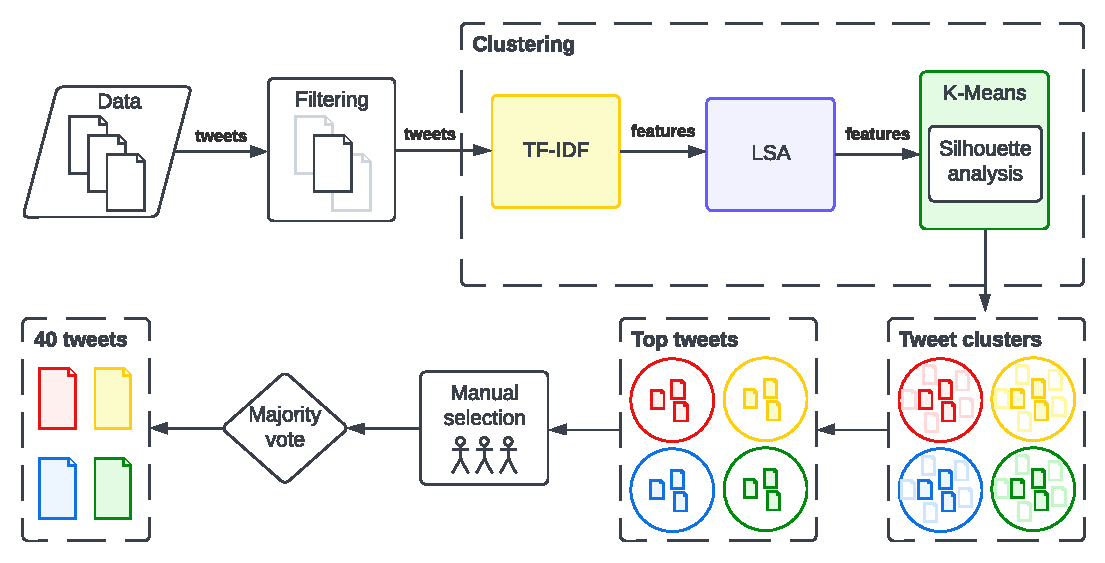
\includegraphics[width=\textwidth]{Figures/clustering.pdf}
    \caption{Flow diagram that visualizes how we perform content analysis to cluster and select the tweets for our survey study.}
    \label{fig:clustering}
\end{figure}

\subsection{Procedure}
We use LimeSurvey\footnote{\url{https://www.limesurvey.org/}} as our survey tool.
%
The survey first presents the informed consent policy and excludes participants that do not agree with it.
%
Next, we show introductory texts to the participants to explain what we will expect from them and to explain the structure of the survey.
%
Using the ME scale, we first present a warm-up task where the participants need to estimate different line lengths to get familiar with using the ME scale.
%
Then, we randomly present 40 scenarios representing the TP, TN, FP, FN, and rejection scenarios (with eight scenarios per type).
%
Each scenario contains several questions with the same structure.
%
The first question is whether participants think the post is hateful (yes/no).
%
The second question is whether participants agree, disagree, or are neutral with SocialNet's decision.
%
In the case of nonneutral, we ask a third question about the degree to which participants agree or disagree with the machine's decisions, using either the ME or 100-level scale, depending on their group.
%
There is no time limit for answering the questions, and all data is anonymous.
%
Finally, we will inform the participants not to put identifiers in their answers.
%
Refer to \autoref{sec:appendix} for all presentation texts, the informed consent, and some scenario examples.

\noindent\customtextbox{
    \begin{itemize}[leftmargin=*, label={}]
        \item \textbf{Step 1: provide informed consent}
              \begin{itemize}
                  \item Show the informed consent (with checkboxes for giving consent).
                  \item Proceed to the next step only for the participants who give consent.
              \end{itemize}
        \item \textbf{Step 2: introduction}
              \begin{itemize}
                  \item Show introductory text about what is expected from the participant.
                  \item We split all participants up into two groups.
                  \item The first group first uses the ME scale to rate all scenarios.
                  \item The second group first uses the 100-level scale to rate all scenarios.
                  \item Explanation of the scale.
              \end{itemize}
        \item \textbf{Step 3: two attention checks}
              \begin{itemize}
                  \item Two simple attention checks where we ask the participant to select one option (shuffled through all scenarios).
              \end{itemize}
        \item \textbf{Step 4a: ME practice phase (when ME is used)}
              \begin{itemize}
                  \item To let participants learn how to use ME, we first run a practice phase where we shuffle and present 5 different line lengths.
                  \item Each participant needs to estimate the line length using any positive value.
              \end{itemize}
        \item \textbf{Step 4b: all scenarios using the scale (ME or 100-level)}
              \begin{itemize}
                  \item Show 40 different scenarios in random order: 8 TP, 8 TN, 8 FP, 8 FN, and 8 rejection.
              \end{itemize}
        \item \textbf{Step 5: finish}
              \begin{itemize}
                  \item Show a thank you message and redirect the users to Prolific to complete the task.
              \end{itemize}
    \end{itemize}
}

\section{Analysis}
\label{sec:survey-analysis}
First, we calculate the value ratios of the TP, TN, FP, FN, and rejection scenarios in hate speech detection using the survey's results.
%
Second, we analyze the quality of our survey method by looking at two aspects: reliability and validity.

\subsection{Value ratios}
\label{sec:analysis-values}
The survey study aims to determine value ratios of the TP, TN, FP, FN, and rejection scenarios in the context of hate speech detection.
%
The metric from section \ref{sec:value-metric} takes these numerical values as input to calculate the optimal rejection threshold.
%
We do not need to know the absolute values but only the relative values.
%
For example, if we set all values to 1, we retrieve the same optimal rejection threshold as setting all values to 1000.
%
We use a bipolar scale for question 3 in the survey since we ask the participants the degree to which they agree, disagree, or are neutral with the decision of SocialNet.
%
For both scales, we will convert disagreement values to negative values, neutral values to 0, and agreement values to positive values.
%
Since we found that the data of both scales is skewed after conducting the pilot survey, we first apply the median to the individual questions' results.
%
Then we calculate the mean value over the resulting values to retrieve the final aggregated value ratios.
%
For example, to calculate the aggregated $V_{tp}$ values for both scales, we use:
\begin{align*}
    V_{tp}^{ME} = \frac{1}{n} \sum_{i=1}^{n} r_{i, tp}^{ME}   & \quad  \parbox{35em}{\footnotesize where $n$ is the total number of all participants for TP scenarios and $r_{i, tp}^{ME}$ is the  \\median response value of TP question number $i$ rated with the ME scale.}\\
    V_{tp}^{100} = \frac{1}{n} \sum_{i=1}^{n} r_{i, tp}^{100} & \quad  \parbox{35em}{\footnotesize where $n$ is the total number of all participants for TP scenarios and $r_{i, tp}^{100}$ is the \\median response value of TP question number $i$ rated with the 100-level scale.}
\end{align*}
%
We apply the same calculations for the remaining scenario types.
%
The results should give us an understanding of how the participants feel towards the different scenarios: TP, TN, FP, FP, and rejection.
%
We define the value ratios we need for the metric using the aggregated values of the TP, TN, FP, FN, and rejection scenarios rated with the ME scale since the ME scale provides us with ratio data.
%
We will not use the aggregated values of the 100-level scale for our metric since the 100-level scale does not provide ratio data, but we will still present them.

\subsection{Reliability}
Reliability is about whether we can trust our results and if we get consistent results \citep{fitzner2007reliability}.
%
We do this by mainly looking at the inter-rater reliability.
%
Different participants should give approximately the same judgements to the same scenarios.
%
We measure the inter-rater reliability using Krippendorff's alpha \citep{maddalena2017crowdsourcing, krippendorff2004reliability}.
%
We calculate the inter-rater reliability value for the complete survey's data for the normalized ME and 100-level values.
%
We use the inter-rater reliability scores to compare the ME scale with the 100-level scale.
%
We also separately study the inter-rater reliability values for the different types of scenarios (TP, TN, FN, FP, and rejection).
%
This experiment does not consider other types of reliability, such as test-retest reliability.
%
Guaranteeing test-retest reliability would require us to redo the complete experiment at a different time for the same participants, which is infeasible for this project, given the limited time and budget.

\subsection{Validity}
\label{sec:analysis-validity}
Validity is about whether we are measuring the things we want to measure \citep{fitzner2007reliability}.
%
The main goal of this aspect is to validate if we can use the ME technique to measure participants' opinions about hate speech detection scenarios.
%
There are multiple types of validity, but we focus mainly on convergent validity (part of construct validity), content validity, and face validity \citep{fitzner2007reliability}.
%
Construct validity checks whether there is an agreement between a theory and a measurement device or procedure \citep{fitzner2007reliability}.
%
Convergent validity is about the correlation between different measures to see if they measure the same phenomenon \citep{fitzner2007reliability}.
%
Content validity is about letting experts review the proposed research questions and procedure \citep{fitzner2007reliability}.
%
Face validity is a subjective type of validity, and it is about why we think the questions and proposed procedures are valid \citep{fitzner2007reliability}.
%

%
We analyze convergent validity by performing cross-modality validation.
%
Following the approach from \citet{roitero2018fine}, we analyze the correlation between the ME scale and the 100-level scale.
%
We can verify that they measure the same phenomenon if we find that both scales are positively correlated.
%
However, we can also expect a low correlation since the ME scale is a (normalized) unbounded scale and the 100-level scale is bounded.
%
Nevertheless, we think both scales will give similar results, meaning that high ME responses should correspond to high 100-level scale responses and low ME responses to low 100-level scale responses.
%
To guarantee content validity, we let experts (the supervisors of this thesis project) check the pre-registration report before conducting the experiments.
%
We tackled face validity in section \ref{sec:related-work-value-assessment} by arguing why we think the ME technique is suitable for measuring people's opinions about hate speech detection scenarios.
%
We exclude other forms of validity from this experiment because they are irrelevant or infeasible.
%
For example, external validity is about the degree to which the findings can be generalized to other settings or groups \citep{fitzner2007reliability}.
%
We think people with different demographic characteristics perceive hate speech differently since people have other norms and values.
%
We believe that if we conduct this experiment using different groups of participants, we might retrieve different value ratios.
%
Therefore, we decided not to create too many participant inclusion criteria but take a random sample of global social media users.
%
We would have to experiment with multiple groups with different demographic characteristics to guarantee external validity.
%
We left this for future work to investigate in full detail.
%
However, we still try to analyze if we can find any differences between participants with different demographic characteristics in the dataset we retrieve (refer to section \ref{sec:analysis-demographic}).

\subsection{Demographics}
\label{sec:analysis-demographic}
As we conduct the survey study only once for a group of participants, among which 50\% are men and 50\% are women, the remaining demographic characteristics can be quite diverse.
%
Nevertheless, we are still curious if there are any significant statistical differences between groups of participants with different demographic characteristics as we expect that demographic characteristics influence people's perception of hate speech and how we should deal with it.
%
Therefore, we apply several statistics to the results of each scenario to analyze if we can find differences between different demographic groups.
%
Prolific provides information about the demographic characteristics of the participants, out of which we analyze four variables: nationality, age, student (whether they are still a student or not), and gender.
%
We have multiple groups (more than two) for the variables nationality and age (different age intervals) and two groups for the variables student and gender.
%
We apply either analysis of variance (ANOVA) (parametric) or Kruskal-Wallis (non-parametric) when we have more than two groups and apply an unpaired two-samples t-test (parametric) or the Mann-Whitney U Test (non-parametric) when we have exactly two groups.
%
First, we check if we can apply the parametric statistics by checking if their assumptions hold in our dataset.
%
If not, then we use the non-parametric tests.
%
We apply ANOVA and the t-test when the data meets the following three conditions: homogeneity of variance (each population has the same variance), normality (normal distribution of the error), and independence (the observations are independent of each other) \citep{howell2012statistical}.
%
We use Bartlett's test of homogeneity of variances and the Shapiro-Wilk test of normality to check if we can apply ANOVA and the t-test.
%
We obey the independence condition since we collect the data of all participants of our survey study Independently.
%
Although ANOVA and the t-test can be robust to violations of the homogeneity of variances and the normality assumptions \citep{howell2012statistical}, we decide to use the non-parametric alternatives instead to prevent us from getting unreliable results.
\chapter{Results}
\label{ch:results}
This chapter presents the results of the survey study (chapter \ref{ch:survey}) and the experiments with the value-sensitive rejector (chapter \ref{ch:rejector}).
%
We first present the results of the survey study as the experiments with the value-sensitive rejector depend on the outcomes of the survey study.
%

%
The goal of the survey study was to retrieve the value ratios of TP, TN, FP, FN, and rejected predictions in hate speech detection from the perspective of the social media user.
%
We retrieved the value ratios using the ME scale.
%
We validated the ME scale by conducting a separate survey using a bounded scale of 100 levels, called the 100-level scale.
%
We defined three goals of the experiments with the value-sensitive rejector.
%
First, we want to analyze how the rejector behaves on different models and datasets.
%
Second, we want to find out if rejecting predictions increases the utilities of the ML models in terms of the value of our value-sensitive metric.
%
Finally, we want to compare the value-sensitive metric against machine metrics such as accuracy.
%

%
Section \ref{sec:results-survey-study} covers the results of the complete survey study that we collected after conducting the pilot survey, and section \ref{sec:results-rejector} covers the results of the experiments with the value-sensitive rejector.

\section{Survey study}
\label{sec:results-survey-study}
We collected the responses of all participants to all scenarios for both surveys: one group that uses the ME scale and another that uses the 100-level scale.
%
All participants had to answer two/three questions per scenario, dependent on the choice of the second question.
%

%
The first question asked whether the participant found the content of the social media post hateful or not.
%
Figure \ref{fig:hatefulness} presents the results of the first question by showing the percentages of participants who find the content hateful or not hateful for each scenario.
%
We summed the ME and the 100-level survey responses since this question was the same for both surveys.
%
Most participants agreed with the ground truth label of the social media posts.
%
Please note that according to the ground truth label, REJ1, REJ2, REJ5, and REJ6 are hateful, and REJ3, REJ4, REJ7, and REJ8 are not hateful.
%
So most participants found the posts used in the TP and FN scenarios hateful and those used in TN and FP scenarios not hateful.
%
For the rejection scenarios, most found the posts of REJ1, REJ2, and REJ6 hateful and REJ3, REJ4, and REJ8 not hateful.
%
However, we found three posts where a significant number of participants tended to disagree with the ground truth label (more than or equal to 40\%): FN5, REJ5, and REJ7.
%

%
The second and third questions asked whether the participant agreed/disagreed or was neutral about SocialNet's decision and to what degree.
%
Figure \ref{fig:boxplots} shows the response values to the second and third questions of all scenarios for both scales.
%
Participants generally agreed with the TP and TN scenarios and disagreed with the FP, FN, and rejection scenarios.
%
For both scales, participants disagreed the most with scenarios FN3 and FN7 and agreed the most with scenarios TN3 and TN6.
%
Scenario FN4 was an exception, as some participants agreed with the scenario for both scales.
%

%
The following sections tackle the different parts of the survey analysis: section \ref{sec:results-value-ratios} presents the value ratios required for our value-sensitive rejector, section \ref{sec:results-reliability} presents the reliability analysis, and section \ref{sec:results-validity} the validity analysis.
%
Finally, section \ref{sec:results-demographics} shows the results of the demographic analysis.
%

%
\begin{figure}[t]
    \centering
    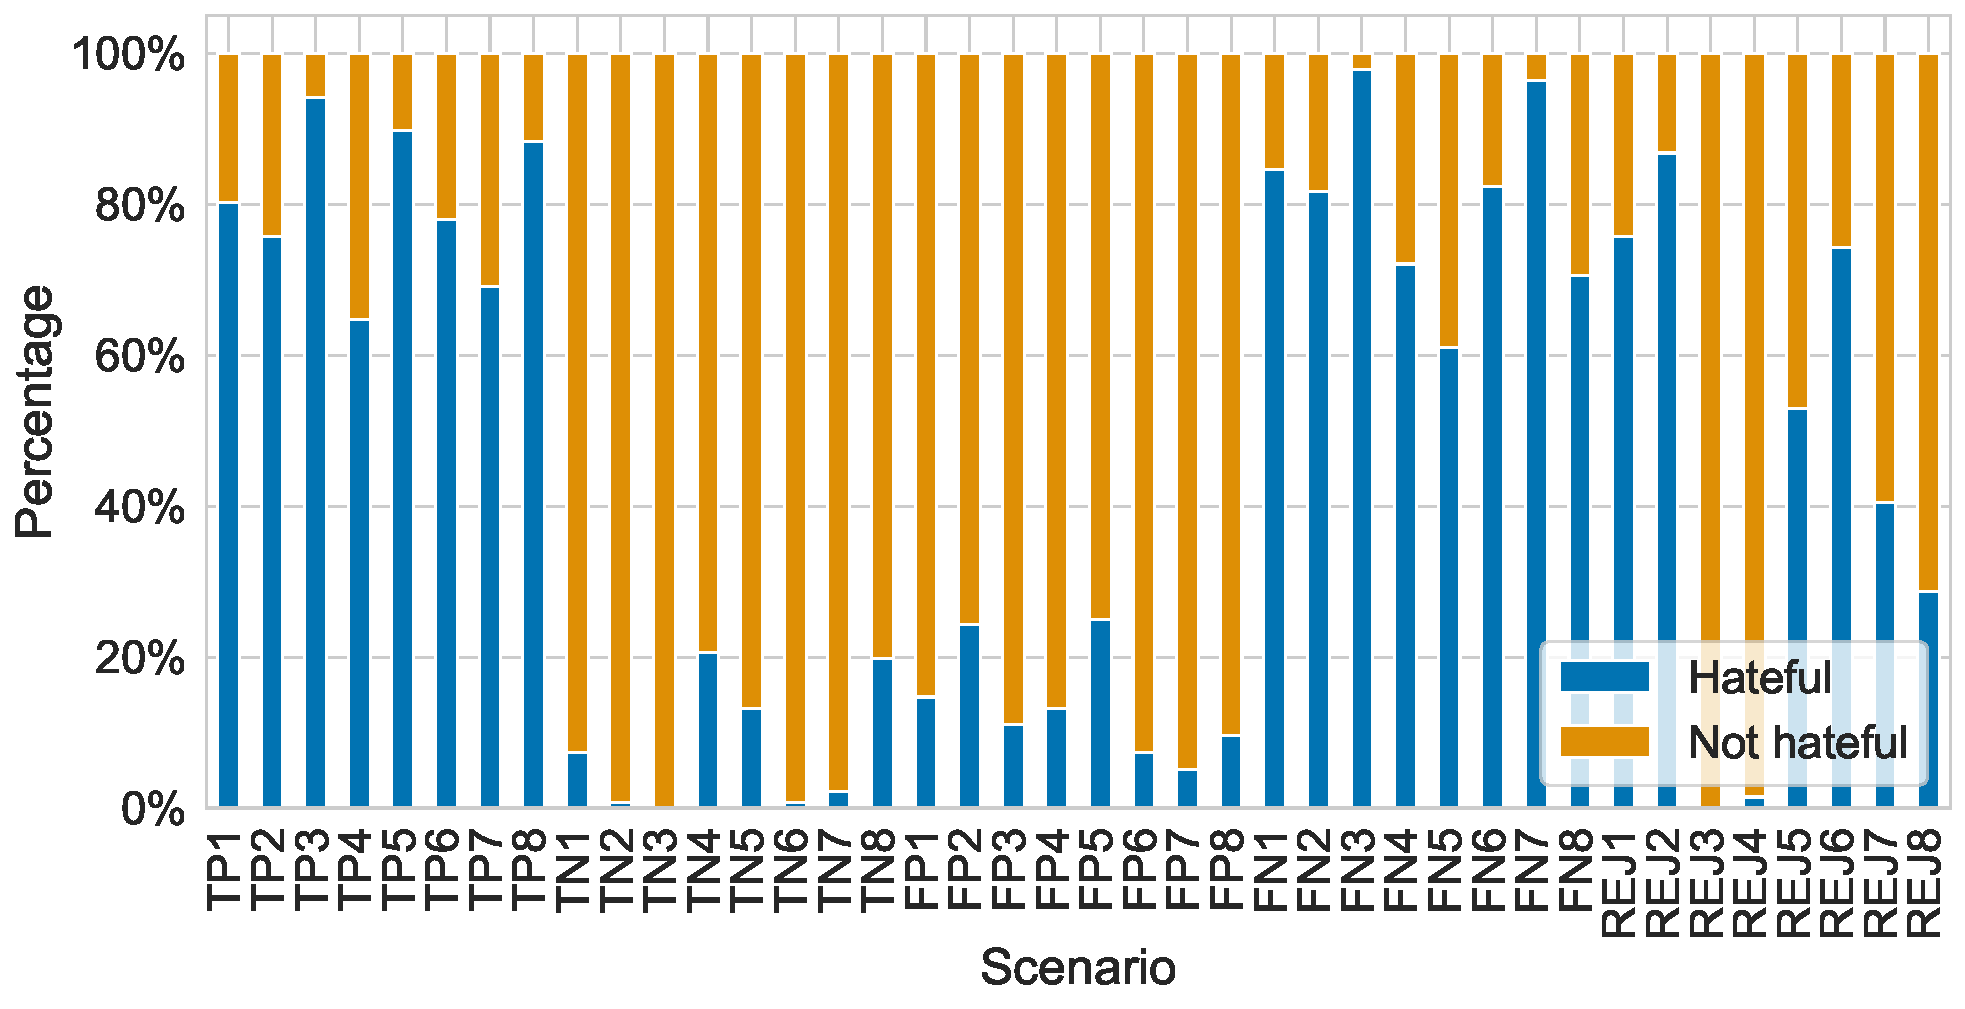
\includegraphics[scale=.4]{Figures/hatefulness.pdf}
    \caption{Stacked bar charts that show the percentages of participants who find the content of the social media post used in the scenarios hateful or not hateful. Each bar is a summation of the responses to both surveys, as this question was the same for both.}
    \label{fig:hatefulness}
\end{figure}
\begin{figure}[h]
    \centering
    \begin{subfigure}[b]{\textwidth}
        \centering
        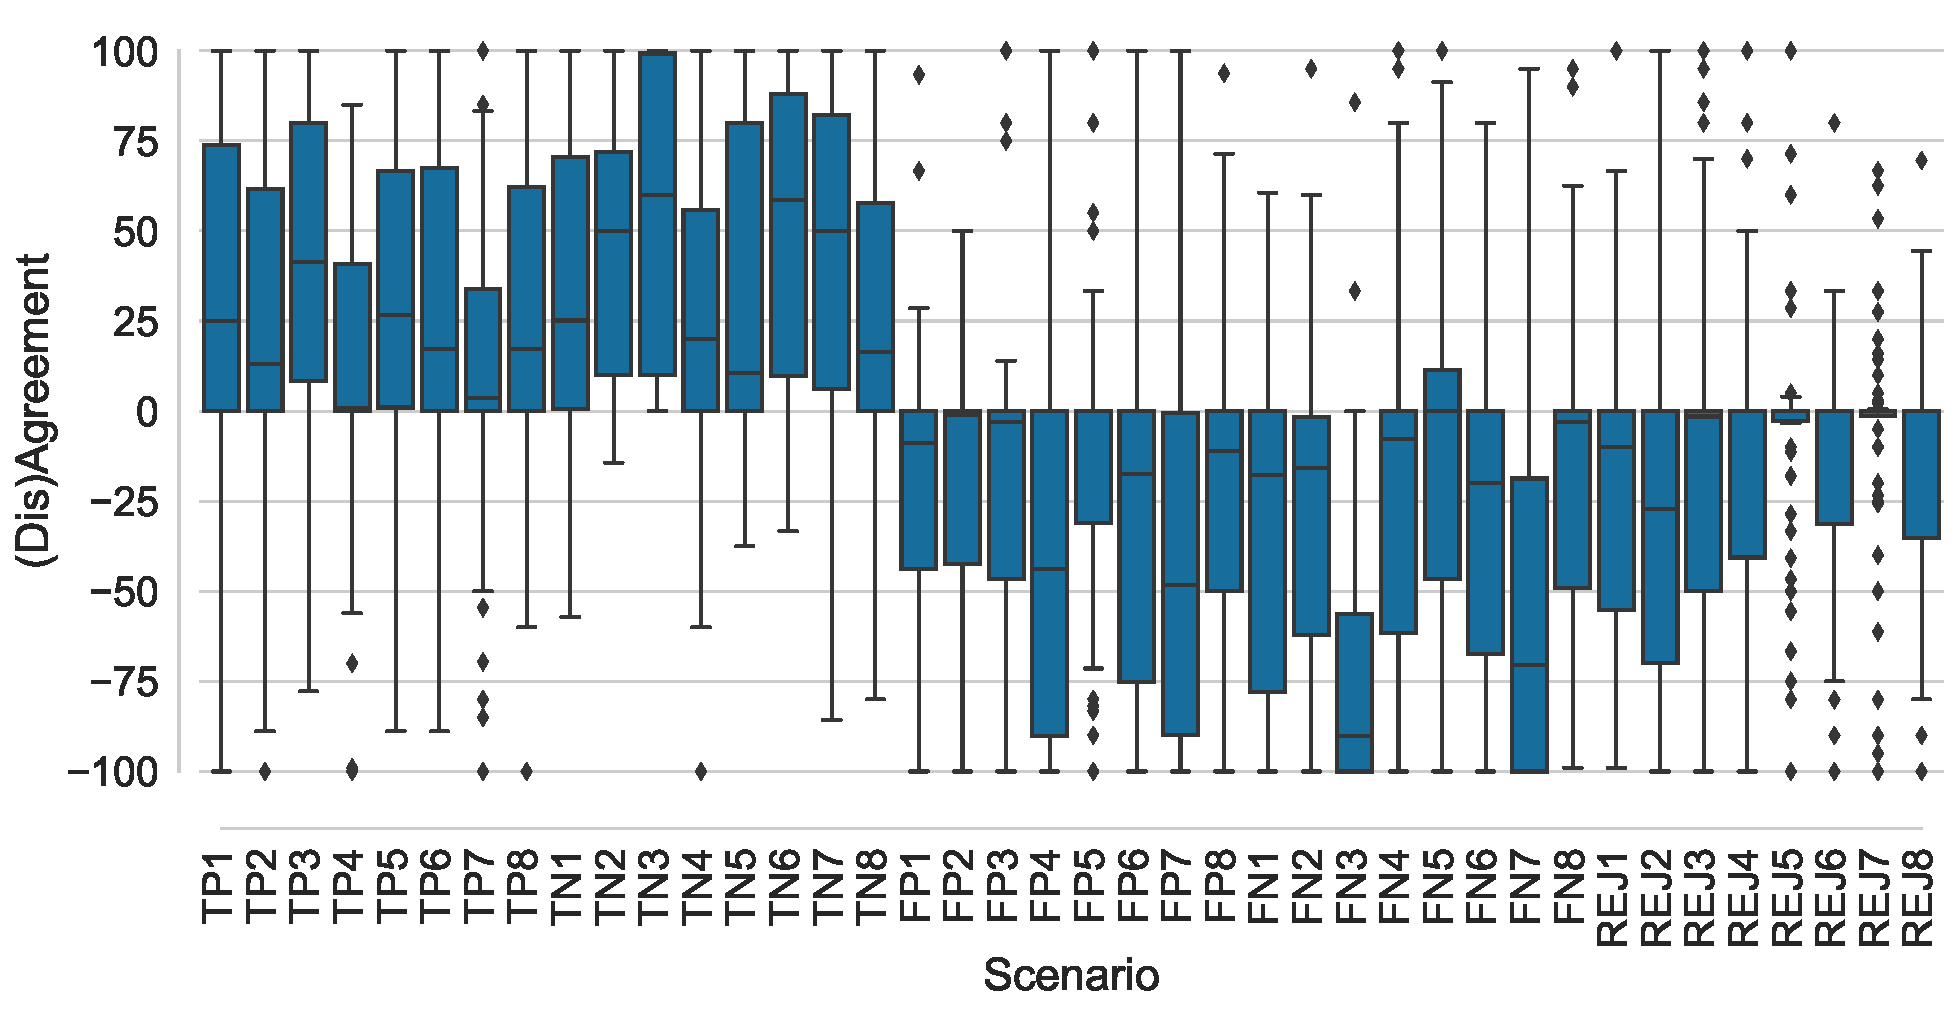
\includegraphics[scale=.4]{Figures/boxplots-ME.pdf}
        \caption{ME scale}
        \label{fig:boxplots-me}
    \end{subfigure}
    \begin{subfigure}[b]{\textwidth}
        \centering
        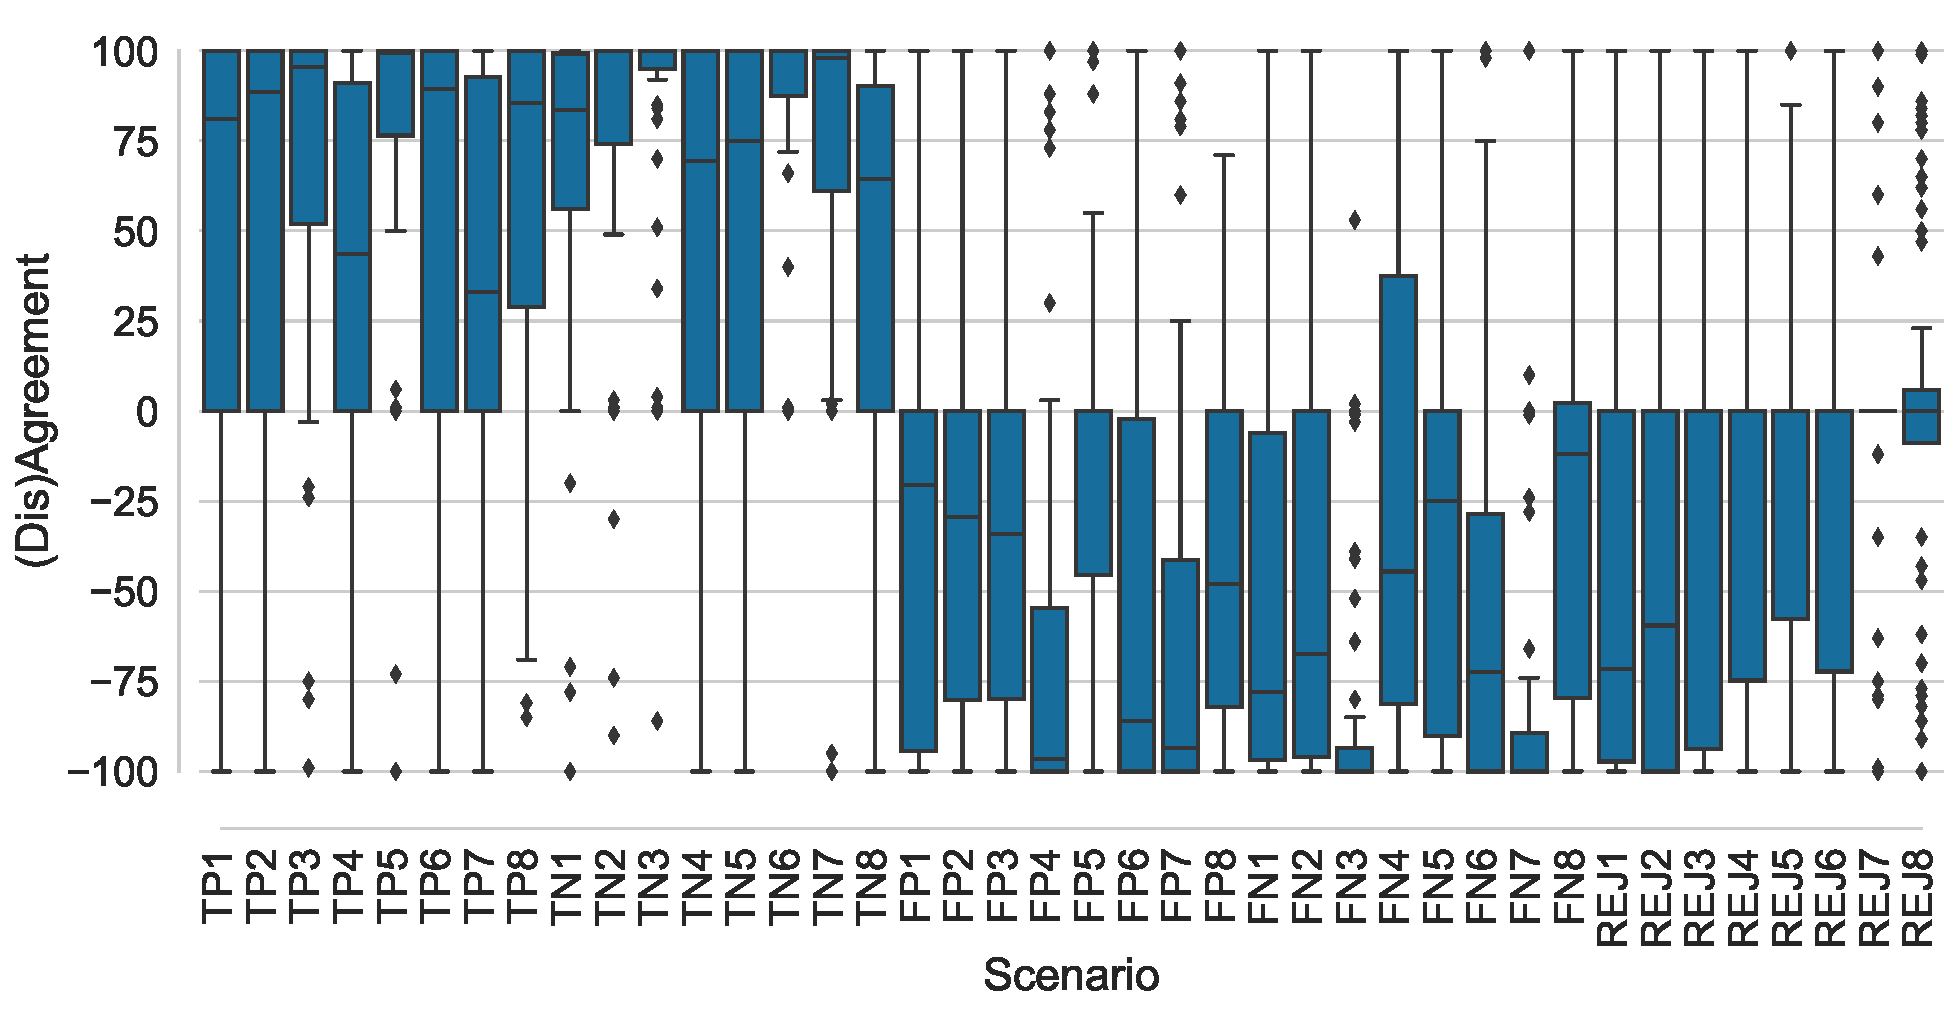
\includegraphics[scale=.4]{Figures/boxplots-100-level.pdf}
        \caption{100-level scale}
        \label{fig:boxplots-100-level}
    \end{subfigure}
    \caption{Boxplots of the responses of all participants to all scenarios for both scales.}
    \label{fig:boxplots}
\end{figure}

\subsection{Value ratios}
\label{sec:results-value-ratios}
We need the value ratios between TP, TN, FP, FN, and rejected predictions in the context of hate speech detection to use our value-sensitive rejector from chapter \ref{ch:rejector} for calculating the optimal rejection threshold.
%
We calculated the value ratios following the approach from section \ref{sec:analysis-values}.
%
Table \ref{tab:values-reliability} shows the resulting values ($v$) from the ME and the 100-level surveys.
%
Positive and negative values indicate agreement and disagreement, respectively.
%
For both scales, participants disagreed the most with the FN scenarios and agreed the most with the TN scenarios.
%
The final values of both scales follow the same order: $V_{fn} < V_{fp} < V_{r} < V_{tp} < V_{tn}$.
%
Participants give the highest absolute response values to the TN scenarios.
%
We also observed that participants provided greater absolute response values to the TP and TN scenarios than to the FP and FN scenarios.
%
\begin{table}[t]
    \small
    \centering
    \begin{tabular}{lcccc}
        \toprule
                           & \multicolumn{2}{c}{\textbf{ME}} & \multicolumn{2}{c}{\textbf{100-level}}                                        \\
        \cmidrule(l){2-3} \cmidrule(l){4-5}
                           & $\boldsymbol{\alpha}$           & $\textbf{v}$                           & $\boldsymbol{\alpha}$ & $\textbf{v}$ \\
        \midrule
        \textbf{TP}        & 0.07                            & 18.15                                  & 0.04                  & 77.00        \\
        \textbf{TN}        & 0.10                            & 36.32                                  & 0.11                  & 86.31        \\
        \textbf{FP}        & 0.39                            & -16.69                                 & 0.07                  & -51.00       \\
        \textbf{FN}        & 0.92                            & -28.08                                 & 0.14                  & -62.43       \\
        \textbf{Rejection} & -0.31                           & -4.82                                  & 0.07                  & -16.37       \\
        \midrule
        \textbf{All}       & 0.78                            & ---                                    & 0.44                  & ---          \\
        \bottomrule
    \end{tabular}
    \caption{Krippendorff's alpha ($\alpha$) and the scenario values ($v$) for TP, TN, FP, FN, and rejection scenarios for the ME and 100-level scales.}
    \label{tab:values-reliability}
\end{table}

\subsection{Reliability}
\label{sec:results-reliability}
As explained in section \ref{sec:reliability}, we measured the interrater reliability between the participants using Krippendorff's alpha.
%
Table \ref{tab:values-reliability} shows Krippendorff's alpha ($\alpha$) values for both scales.
%
In the last row of the table, we computed the $\alpha$ values over the responses to all scenarios.
%
The ME scale seemed more reliable than the 100-level scale.
%
According to \citet{krippendorff2004reliability}, the results of the ME scale are reliable, while the results of the 100-level scale are likely to be unreliable.
%

%
We also computed the $\alpha$ values for each group of scenarios of the same type (TP, TN, FP, FN, or rejection).
%
Participants using the ME scale tended to agree with each other on the FP and FN scenarios, while they tended to disagree on the rejection scenarios.
%
For the 100-level scale, we see that participants have low agreement on all scenario types.

\subsection{Validity}
\label{sec:results-validity}
We analyzed the validity of the ME method by performing cross-modality validation between the ME and the 100-level scale (refer to section \ref{sec:analysis-validity}).
%
Figure \ref{fig:correlation} shows the correlation between the ME scale and the 100-level scale.
%
The Shapiro-Wilk test of normality showed that both the median (normalized) ME scores and the median 100-level scores do not follow a normal distribution ($p < 0.05$).
%
We calculated the median because when we look at figure \ref{fig:boxplots}, we can see that the data of both scales are skewed and contain many extreme outliers.
% 
We calculated the Spearman and the Kendall correlation statistics as these are non-parametric and, therefore, do not require the normality assumption.
%
Spearman returned a 0.98 and Kendall a 0.89 correlation between the ME and the 100-level scales ($p < 0.05$), indicating that both scales are highly correlated.

\begin{figure}
    \centering
    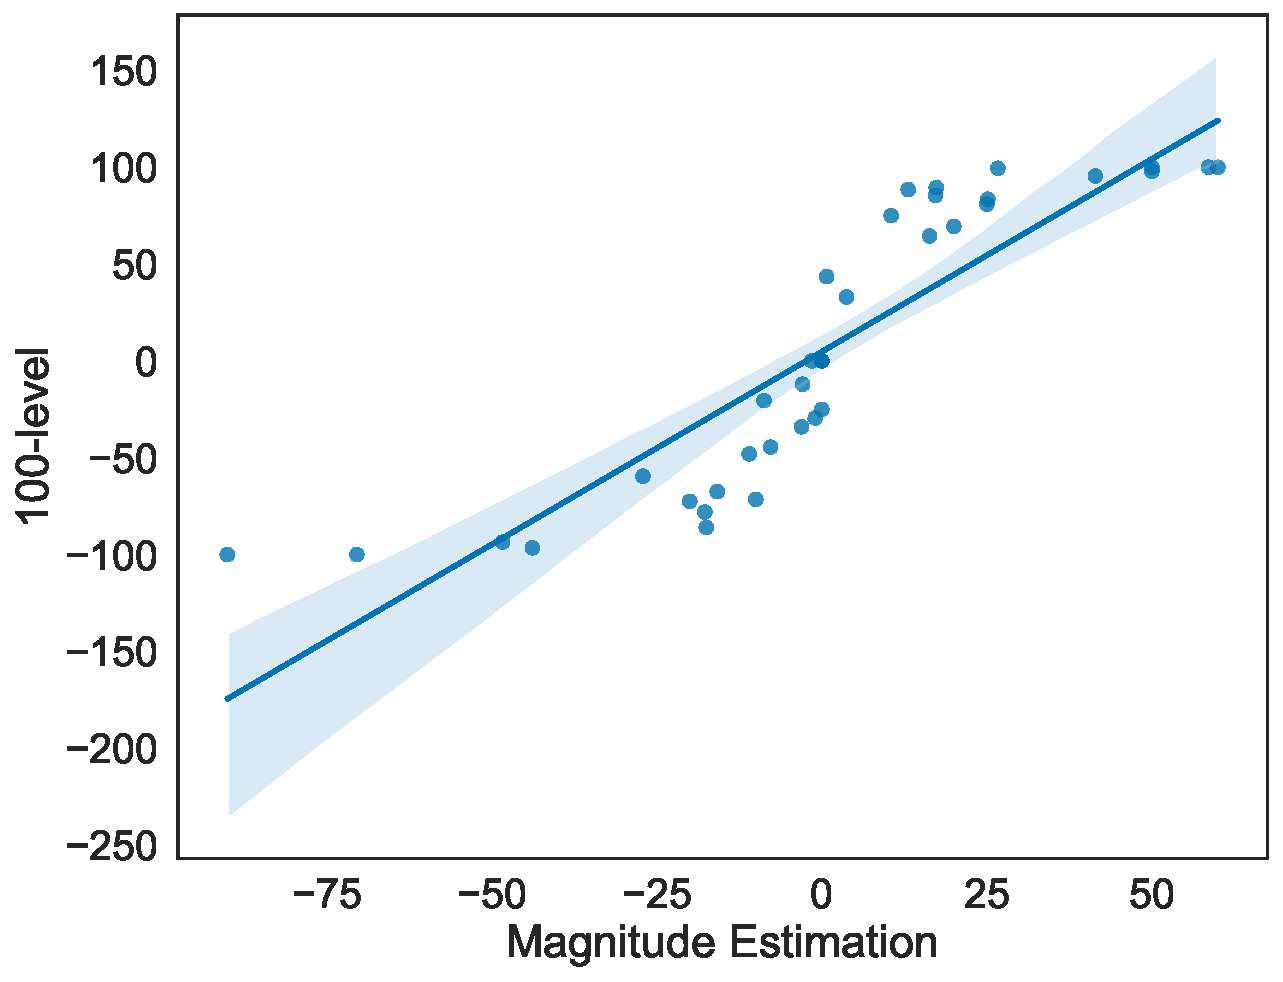
\includegraphics[scale=.4]{Figures/correlation.pdf}
    \caption{Correlation plot between the median normalized magnitude estimates and the median 100-level scores per question.}
    \label{fig:correlation}
\end{figure}

\subsection{Demographics}
\label{sec:results-demographics}
We followed the approach from section \ref{sec:analysis-demographic} to analyze whether statistically significant differences exist between groups with different demographic characteristics.
%
We focused on six features: sex, student, continent, nationality, language, and ethnicity.
%

%
We only used non-parametric statistical tests to analyze the demographic differences for two reasons.
%
First, we found that the assumptions of normality and homogeneity of variances were violated in our dataset when looking at the different groups for all features.
%
Second, we found that for most features, except sex, the sample sizes of the feature groups were not equal.
%
We used Mann-Whitney U to verify a significant difference between the two groups, and we used Kruskal-Wallis for more than two groups.
%

%
Table \ref{tab:results-differences-ind} shows the resulting p values for all scenarios and all features.
%
We found that there are no significant differences between men and women.
%
We found only three scenarios with significant differences for the student and continent features.
%
We found the most significant differences when looking at nationality and language.
%
We observed five scenarios with non-hateful posts and ten scenarios with hateful posts where there is at least one feature with significant differences between the groups.
%
Scenarios FP7 and REJ4 have the most features (4) with significant differences.
%
Scenarios TP6, FN5, and REJ1 have the second most features (2) with significant differences.
%

%
Table \ref{tab:results-differences-grp} shows the p values of the statistical tests for the aggregated scenarios (TP, TN, FP, FN, and rejection) and all features.
%
We aggregated the scores by calculating the mean response value to all scenarios of the same type, e.g. TP, for each participant.
%
Then we applied the statistical tests to the aggregated scores.
%
We found the most significant differences in the aggregated scores of the FP scenarios.
%

%
Finally, we conducted pairwise Mann-Whitney U tests to check if there are any significant differences between pairs of groups for the multi-group features: nationality, language, and ethnicity.
%
Tables \ref{tab:results-pairwise-nationality}, \ref{tab:results-pairwise-language}, and \ref{tab:results-pairwise-ethnicity} present the resulting p values of the pairwise Mann-Whitney U tests for the features of nationality, language, and ethnicity, respectively.
%
We did not find many pairwise significant differences for most of these scenarios and the three features.
%
We found the most pairwise differences (four out of the six pairs) for scenario FN5 and the nationality feature.
%
\begin{table}
    \small
    \centering
    \begin{tabular}{lccc|ccc}
        \toprule
                      & \multicolumn{3}{c}{\textbf{Two groups}} & \multicolumn{3}{c}{\textbf{More than two groups}}                                                                                                                                                                       \\
        \midrule
                      & \multicolumn{1}{c}{\textbf{Sex}}        & \multicolumn{1}{c}{\textbf{Student}}              & \multicolumn{1}{c}{\textbf{Continent}} & \multicolumn{1}{c}{\textbf{Nationality}} & \multicolumn{1}{c}{\textbf{Language}}  & \multicolumn{1}{c}{\textbf{Ethnicity}} \\
        \midrule
        \textbf{TP1}  & 0.506                                   & 0.371                                             & 0.982                                  & 0.095                                    & 0.117                                  & 0.108                                  \\
        \textbf{TP2}  & 0.268                                   & 0.201                                             & 0.387                                  & 0.300                                    & 0.330                                  & 0.464                                  \\
        \textbf{TP3}  & 0.680                                   & 0.276                                             & 0.577                                  & 0.160                                    & \cellcolor[HTML]{EFEFEF}\textbf{0.046} & 0.138                                  \\
        \textbf{TP4}  & 0.756                                   & 0.441                                             & 0.774                                  & 0.137                                    & 0.175                                  & 0.568                                  \\
        \textbf{TP5}  & 0.392                                   & \cellcolor[HTML]{EFEFEF}\textbf{0.011}            & 0.387                                  & 0.152                                    & 0.106                                  & 0.341                                  \\
        \textbf{TP6}  & 0.260                                   & 0.097                                             & 0.682                                  & \cellcolor[HTML]{EFEFEF}\textbf{0.002}   & \cellcolor[HTML]{EFEFEF}\textbf{0.006} & 0.215                                  \\
        \textbf{TP7}  & 0.342                                   & 0.730                                             & 0.059                                  & 0.241                                    & 0.400                                  & 0.238                                  \\
        \textbf{TP8}  & 0.495                                   & \cellcolor[HTML]{EFEFEF}\textbf{0.015}            & 0.246                                  & 0.568                                    & 0.387                                  & 0.190                                  \\
        \textbf{TN1}  & 0.430                                   & 0.480                                             & 0.554                                  & 0.307                                    & 0.260                                  & 0.449                                  \\
        \textbf{TN2}  & 0.567                                   & 0.382                                             & 0.633                                  & 0.595                                    & 0.716                                  & 0.833                                  \\
        \textbf{TN3}  & 0.393                                   & 0.866                                             & 0.766                                  & 0.443                                    & 0.298                                  & 0.432                                  \\
        \textbf{TN4}  & 0.104                                   & 0.171                                             & 0.059                                  & 0.245                                    & 0.251                                  & 0.201                                  \\
        \textbf{TN5}  & 0.290                                   & 0.199                                             & 0.964                                  & 0.304                                    & 0.177                                  & 0.296                                  \\
        \textbf{TN6}  & 0.521                                   & 0.510                                             & 0.608                                  & 0.815                                    & 0.748                                  & 0.600                                  \\
        \textbf{TN7}  & 0.224                                   & 0.878                                             & \cellcolor[HTML]{EFEFEF}\textbf{0.050} & 0.108                                    & 0.223                                  & 0.314                                  \\
        \textbf{TN8}  & 0.191                                   & 0.417                                             & 0.327                                  & 0.168                                    & 0.761                                  & 0.872                                  \\
        \textbf{FP1}  & 0.270                                   & 0.545                                             & 0.065                                  & 0.093                                    & 0.333                                  & 0.174                                  \\
        \textbf{FP2}  & 0.337                                   & 0.114                                             & 0.155                                  & \cellcolor[HTML]{EFEFEF}\textbf{0.008}   & 0.164                                  & 0.195                                  \\
        \textbf{FP3}  & 0.561                                   & 0.509                                             & 0.889                                  & 0.793                                    & 0.725                                  & 0.205                                  \\
        \textbf{FP4}  & 0.278                                   & 0.860                                             & 0.908                                  & 0.267                                    & 0.186                                  & 0.344                                  \\
        \textbf{FP5}  & 0.847                                   & 0.445                                             & 0.220                                  & 0.269                                    & 0.554                                  & 0.194                                  \\
        \textbf{FP6}  & 0.774                                   & 0.266                                             & 0.555                                  & 0.758                                    & 0.409                                  & 0.486                                  \\
        \textbf{FP7}  & 0.391                                   & 0.784                                             & \cellcolor[HTML]{EFEFEF}\textbf{0.015} & \cellcolor[HTML]{EFEFEF}\textbf{0.026}   & \cellcolor[HTML]{EFEFEF}\textbf{0.020} & \cellcolor[HTML]{EFEFEF}\textbf{0.010} \\
        \textbf{FP8}  & 0.624                                   & 0.837                                             & 0.681                                  & 0.544                                    & 0.225                                  & 0.705                                  \\
        \textbf{FN1}  & 0.337                                   & 0.213                                             & 0.317                                  & 0.261                                    & 0.668                                  & 0.558                                  \\
        \textbf{FN2}  & 0.791                                   & 0.928                                             & 0.759                                  & 0.967                                    & 0.974                                  & 0.823                                  \\
        \textbf{FN3}  & 0.990                                   & 0.752                                             & 0.480                                  & 0.504                                    & 0.455                                  & 0.182                                  \\
        \textbf{FN4}  & 0.511                                   & 0.573                                             & 0.450                                  & 0.549                                    & 0.856                                  & 0.965                                  \\
        \textbf{FN5}  & 0.306                                   & 0.467                                             & 0.802                                  & \cellcolor[HTML]{EFEFEF}\textbf{0.001}   & \cellcolor[HTML]{EFEFEF}\textbf{0.009} & 0.349                                  \\
        \textbf{FN6}  & 0.109                                   & 0.113                                             & 0.928                                  & \cellcolor[HTML]{EFEFEF}\textbf{0.012}   & 0.084                                  & 0.436                                  \\
        \textbf{FN7}  & 0.871                                   & 0.677                                             & 0.093                                  & 0.107                                    & \cellcolor[HTML]{EFEFEF}\textbf{0.046} & 0.148                                  \\
        \textbf{FN8}  & 0.776                                   & \cellcolor[HTML]{EFEFEF}\textbf{0.009}            & 0.819                                  & 0.949                                    & 0.363                                  & 0.117                                  \\
        \textbf{REJ1} & 0.799                                   & 0.734                                             & 0.544                                  & \cellcolor[HTML]{EFEFEF}\textbf{0.021}   & \cellcolor[HTML]{EFEFEF}\textbf{0.012} & 0.168                                  \\
        \textbf{REJ2} & 0.644                                   & 0.202                                             & 0.741                                  & 0.295                                    & 0.258                                  & 0.749                                  \\
        \textbf{REJ3} & 0.803                                   & 0.815                                             & 0.108                                  & 0.425                                    & 0.482                                  & 0.133                                  \\
        \textbf{REJ4} & 0.985                                   & 1.000                                             & \cellcolor[HTML]{EFEFEF}\textbf{0.002} & \cellcolor[HTML]{EFEFEF}\textbf{0.014}   & \cellcolor[HTML]{EFEFEF}\textbf{0.036} & \cellcolor[HTML]{EFEFEF}\textbf{0.002} \\
        \textbf{REJ5} & 0.133                                   & 0.994                                             & 0.570                                  & 0.111                                    & \cellcolor[HTML]{EFEFEF}\textbf{0.036} & 0.090                                  \\
        \textbf{REJ6} & 0.244                                   & 0.195                                             & 0.716                                  & 0.061                                    & 0.166                                  & 0.664                                  \\
        \textbf{REJ7} & 0.911                                   & 0.853                                             & 0.942                                  & 0.997                                    & 0.996                                  & \cellcolor[HTML]{EFEFEF}\textbf{0.020} \\
        \textbf{REJ8} & 0.157                                   & 0.167                                             & 0.944                                  & 0.901                                    & 0.741                                  & 0.108                                  \\
        \bottomrule
    \end{tabular}
    \caption{\textbf{Individual}: an overview of the statistical differences between different groups of participants for various demographic characteristics for each scenario in the ME survey. Each cell contains the p value of either the Mann-Whitney U test for two groups or the Kruskal-Wallis test for more than two groups. The grey cells with bold text indicate significant statistical differences between the groups for that feature and scenario type.}
    \label{tab:results-differences-ind}
\end{table}

\section{Value-sensitive rejection}
\label{sec:results-rejector}
We experimented with our value-sensitive rejector following the approach from section \ref{sec:rejector-application}.
%
We produced a set of predictions for each experimental setup, applied our value-sensitive rejector to each setup, and collected the results for analysis.
%

%
We used all three models (LR, DistilBERT, and CNN) to produce predictions for both the \emph{seen} and \emph{unseen} datasets.
%
Therefore, we ended up with six different sets of predictions.
%
Then, for each set of predictions, we created the PDFs for all predictions of the same type (TP, TN, FP, and FN).
%
The PDFs were necessary for calculating the total value of the models with the reject option.
%
Figures \ref{fig:pdfs-seen} and \ref{fig:pdfs-unseen} show all PDFs for the \emph{seen} and \emph{unseen} datasets, respectively.
%
We observed that all three models were more confident in their correct predictions (TP and TN) than their incorrect predictions (FP and FN) for both the \emph{seen} and \emph{unseen} datasets.
%
All three models were also more confident in their correct predictions for the \emph{seen} dataset than the \emph{unseen} dataset.
%
The CNN and LR models have similar PDFs and seem more calibrated since the PDFs of the correct predictions are skewed towards $1.0$.
%
In contrast, the PDFs of the incorrect predictions follow a more uniform distribution.
%
The DistilBERT model is less calibrated than the other two models.
%
We recognize this in the PDFs of the incorrect predictions in figures \ref{fig:pdfs-seen} and \ref{fig:pdfs-unseen} of the DistilBERT model by looking at the large density values around the high confidence values.
%

% Continu
%
We applied the value-sensitive metric from section \ref{sec:value-metric} to the three models and the two datasets using the PDFs and the ME values ($V_{tp}, V_{tn}, V_{fp}, V_{fn}, \text{ and } V_r$) from the survey.
%
Figure \ref{fig:metric-plots-all-values} presents the total value of all models with the reject option ($V(\tau)$) for all possible rejection thresholds ($\tau \in [0.5, 1.0]$) and the ME values from table \ref{tab:values-reliability}.
%
The diamond-shaped markers indicate the optimal rejection threshold ($\tau_O$) for which the model achieves the highest total value ($V(\tau_O)$).
%
Positive $V(\tau)$ values indicate that the model for rejection threshold $\tau$ is valuable, and negative values indicate that the costs of incorrect accepted and rejected predictions exceed the gains of correct accepted and rejected predictions.
%
For all models, we got $\tau_O \approx 0.5$, meaning that all models achieve the highest total value when all predictions are accepted.
%
Figure \ref{fig:metric-plots-all-values} shows that all models' $V(\tau_O)$ values are greater for the \emph{seen} data than for the \emph{unseen} data.
%
The total value of all models decreases for increasing values of the rejection threshold.
%

%
To further examine how $V(\tau)$ behaves when we only consider punishing incorrect predictions instead of rewarding correct predictions, we decided to apply the metric again, setting $V_{tp}$ and $V_{tn}$ equal to zero.
%
The metric's conditions \ref{for:conditions-fp-fn} and \ref{for:conditions-tp-tn} were still satisfied when we did this.
%
Figure \ref{fig:metric-plots-tptn0} presents the total value ($V(\tau)$) again for the updated values $V_{tp}=0$ and $V_{tn}=0$.
%
We found that $\tau_O$ of all models moved towards $1.0$, meaning that rejecting predictions is now more beneficial for the total value of the models.
%
All models achieve the highest $V(\tau)$ value when $\tau \in [0.7, 0.9]$ for \emph{seen} data and when $\tau \in [0.9, 1.0]$ for \emph{unseen data}.
%

%
Table \ref{tab:metric} shows the specific values of $\tau_O$, the accuracies of the accepted predictions, and the rejection rates (fraction of rejected predictions).
%
The first two rows show that the accuracies of all models dropped when we applied the models to \emph{unseen} data.
%
The last two rows (where $V_{tp}=0$ and $V_{tn}=0$) show that we achieved higher accuracies of accepted predictions for increasing optimal rejection thresholds.
%
For all models, we rejected less than 30\% of all predictions for the \emph{seen} data and a large fraction for the \emph{unseen} data.
%
The DistilBERT model achieved the highest accuracies of accepted predictions for all configurations.
%
For the \emph{seen} data, it achieved an accuracy of accepted predictions of $92.6\%$ while rejecting only $25.2\%$ of all predictions.
%
For the \emph{unseen} data, it rejected the least amount of predictions ($92.3\%$) and achieved the highest accuracy of accepted predictions ($88.1\%$).
%
The CNN model performs the worst for all configurations regarding the accuracy of accepted predictions.
%
The model achieved the highest value for the \emph{unseen} data when all predictions were rejected, indicating that it is not valuable to use the model.

%
Table \ref{tab:metric2} compares the results of our value-sensitive metric with machine metrics like accuracy.
%
For all models, it presents the total value for the optimal rejection thresholds ($V(\tau_O)$), the total value when all predictions are accepted ($V(0)$), and the accuracies when all predictions are accepted.
%
First, we compared the accuracy of the original model with $V(0)$, as in both cases, all predictions were accepted.
%
In the first two rows, both the accuracy and $V(0)$ indicate that the DistilBERT model performed the best for both the \emph{seen} and \emph{unseen} datasets.
%
In the last two rows (where $V_{tp}=0$ and $V_{tn}=0$), both metrics indicate that the DistilBERT model performed the best for the \emph{seen} dataset but got different results for the \emph{unseen} dataset.
%
Then, according to the accuracy, the DistilBERT model performed the best, while the CNN model performed the best according to $V(0)$.
%
All $V(0)$ values in the last row show that none of the models is valuable for \emph{unseen} data when we accept all predictions.
%

%
When we look at the $V(\tau_O)$ values in table \ref{tab:metric2}, we see that all models are valuable for the optimal rejection threshold.
%
The DistilBERT model achieved the highest $V(\tau_O)$ values in all configurations except for the \emph{unseen} data with $V_{tp}=0$ and $V_{tn}=0$, as the LR model achieved a higher total value.
%
This result is interesting as we can see from table \ref{tab:metric} that for the DistilBERT model, the accuracy of the accepted predictions is higher, and the rejection rate is lower than for the LR model.
%
Looking at the last row, we can see that all models become valuable when we adopt the optimal rejection threshold.


\begin{figure}
    \centering
    \begin{subfigure}{.49\textwidth}
        \centering
        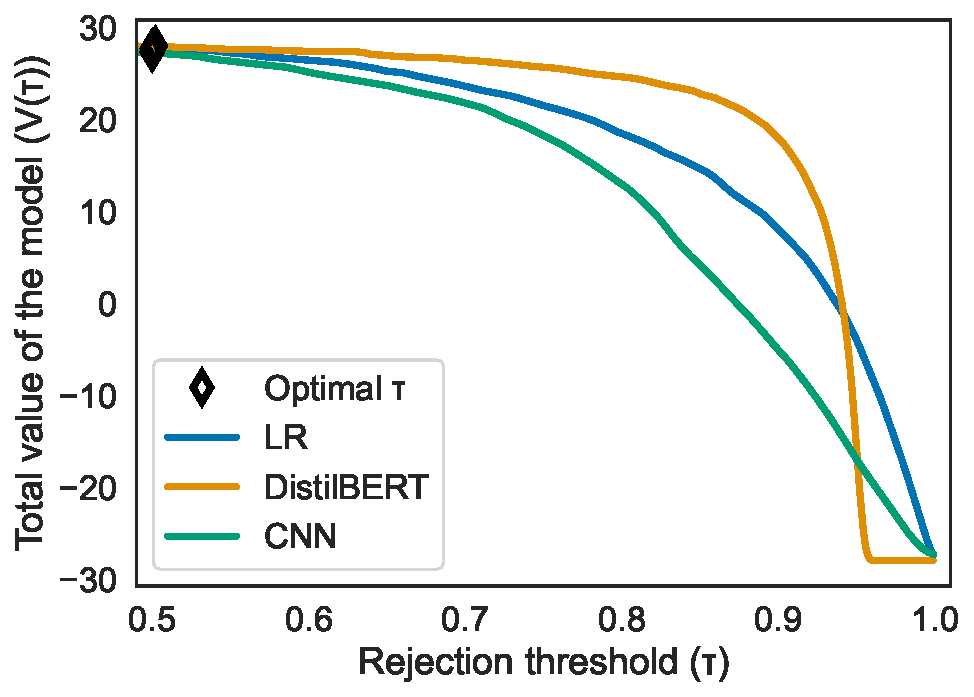
\includegraphics[scale=.4]{Figures/metric-all-values-seen-data.pdf}
        \caption{evaluated on \emph{seen} data}
    \end{subfigure}
    \begin{subfigure}{.49\textwidth}
        \centering
        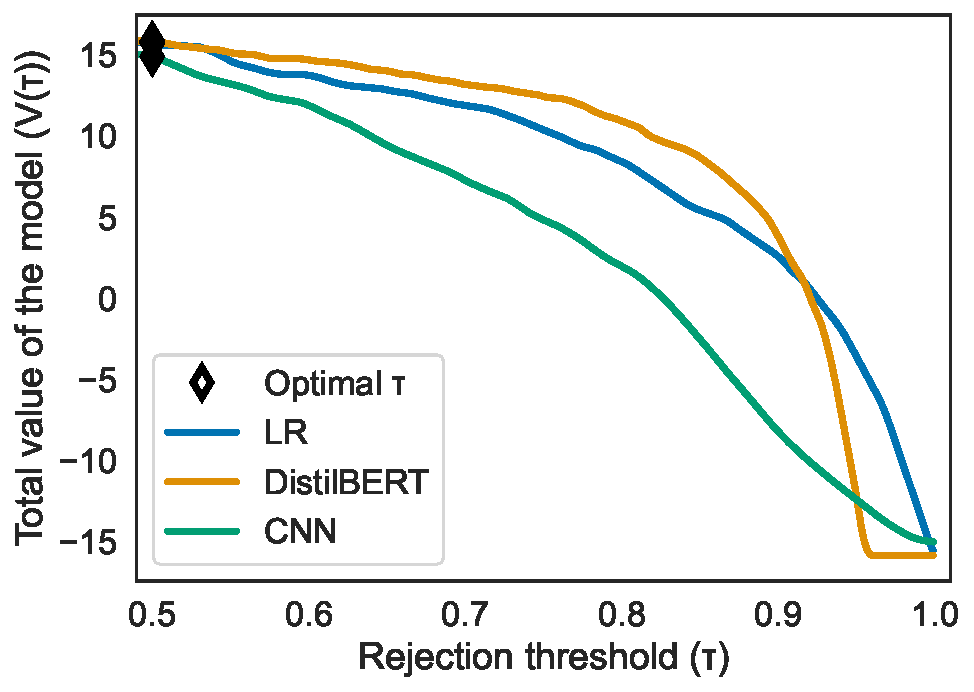
\includegraphics[scale=.4]{Figures/metric-all-values-unseen-data.pdf}
        \caption{evaluated on \emph{unseen} data}
    \end{subfigure}
    \caption{$V(\tau)$ functions of all models with $V_{tp} = 18.15$, $V_{tn} = 36.32$, $V_{fp} = 16.69$, $V_{fn} = 28.08$, $V_r = 4.82$.}
    \label{fig:metric-plots-all-values}
\end{figure}

\begin{figure}
    \centering
    \begin{subfigure}{.49\textwidth}
        \centering
        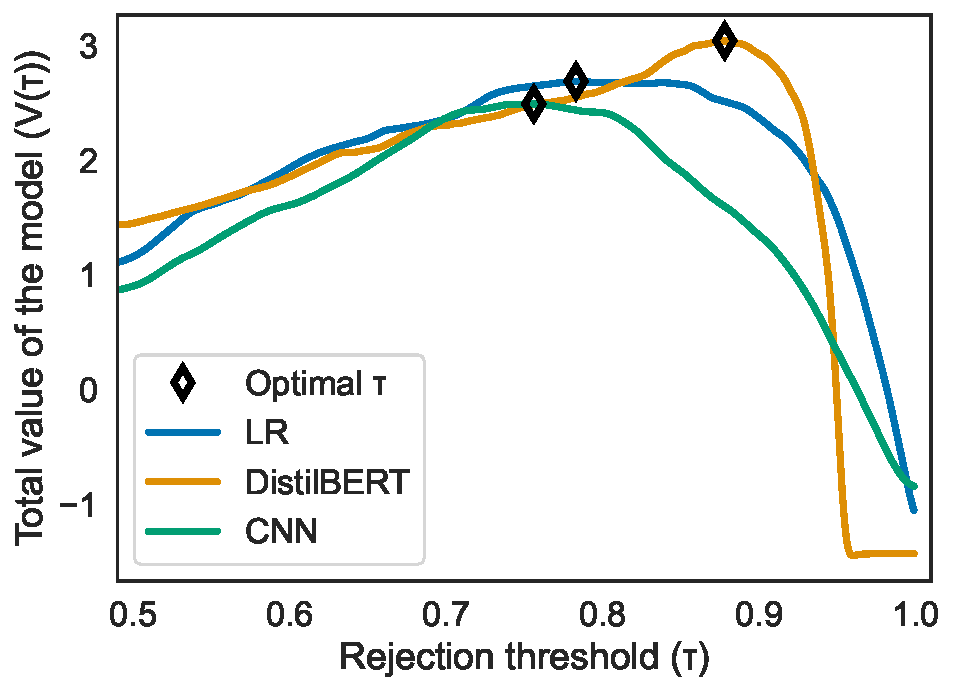
\includegraphics[scale=.4]{Figures/metric-tptn0-seen-data.pdf}
        \caption{evaluated on \emph{seen} data}
    \end{subfigure}
    \begin{subfigure}{.49\textwidth}
        \centering
        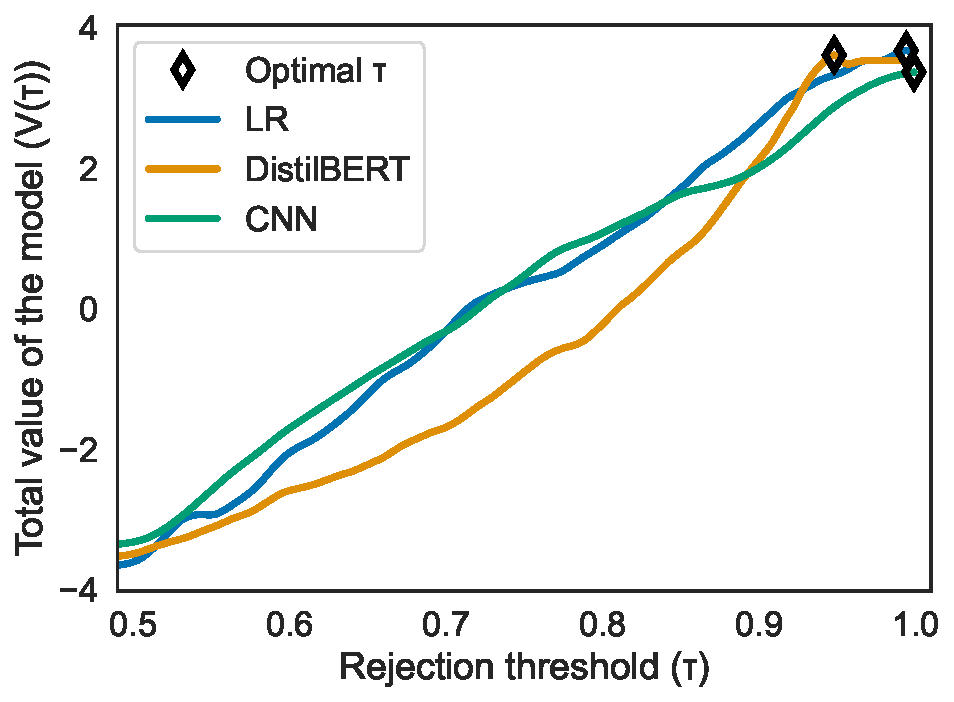
\includegraphics[scale=.4]{Figures/metric-tptn0-unseen-data.pdf}
        \caption{evaluated on \emph{unseen} data}
    \end{subfigure}
    \caption{$V(\tau)$ functions of all models with $V_{tp} = 0.0$, $V_{tn} = 0.0$, $V_{fp} = 16.69$, $V_{fn} = 28.08$, $V_r = 4.82$.}
    \label{fig:metric-plots-tptn0}
\end{figure}

\begin{table}
    \scriptsize
    \centering
    \setlength\tabcolsep{5pt}
    \begin{tabular}{lcccccccccc}
        \toprule
                                                 & \multicolumn{3}{c}{\textbf{LR}} & \multicolumn{3}{c}{\textbf{DistilBERT}} & \multicolumn{3}{c}{\textbf{CNN}}                                                                                                           \\
        \cmidrule(l){2-4} \cmidrule(l){5-7} \cmidrule(l){8-10}
                                                 & $\boldsymbol{\tau_O}$           & \textbf{Acc}                            & \textbf{RR}                      & $\boldsymbol{\tau_O}$ & \textbf{Acc} & \textbf{RR} & $\boldsymbol{\tau_O}$ & \textbf{Acc} & \textbf{RR} \\
        \midrule
        \textbf{Seen data}                       & 0.500                           & 0.847                                   & 0.000                            & 0.502                 & 0.850        & 0.000       & 0.500                 & 0.835        & 0.000       \\
        \textbf{Unseen data}                     & 0.500                           & 0.640                                   & 0.000                            & 0.500                 & 0.640        & 0.000       & 0.500                 & 0.629        & 0.000       \\
        \midrule
        \textbf{Seen data $(V_{tp}=V_{tn}=0)$}   & 0.783                           & 0.910                                   & 0.250                            & 0.878                 & 0.926        & 0.252       & 0.756                 & 0.898        & 0.278       \\
        \textbf{Unseen data $(V_{tp}=V_{tn}=0)$} & 0.994                           & 0.752                                   & 0.958                            & 0.948                 & 0.881        & 0.923       & 0.999                 & -            & 1.0         \\
        \bottomrule
    \end{tabular}
    \caption{The optimal rejection thresholds ($\tau_O$), the accuracy of the accepted predictions (Acc), and the rejection rates (RR) of all models for both datasets.}
    \label{tab:metric}
\end{table}

\begin{table}
    \scriptsize
    \centering
    \setlength\tabcolsep{5pt}
    \begin{tabular}{lcccccccccc}
        \toprule
                                                 & \multicolumn{3}{c}{\textbf{LR}} & \multicolumn{3}{c}{\textbf{DistilBERT}} & \multicolumn{3}{c}{\textbf{CNN}}                                                                                                                                 \\
        \cmidrule(l){2-4} \cmidrule(l){5-7} \cmidrule(l){8-10}
                                                 & $\boldsymbol{V(\tau_O)}$        & $\boldsymbol{V(0)}$                     & \textbf{Acc}                     & $\boldsymbol{V(\tau_O)}$ & $\boldsymbol{V(0)}$ & \textbf{Acc} & $\boldsymbol{V(\tau_O)}$ & $\boldsymbol{V(0)}$ & \textbf{Acc} \\
        \midrule
        \textbf{Seen data}                       & 27.707                          & 27.707                                  & 0.847                            & 28.001                   & 27.996              & 0.850        & 27.291                   & 27.291              & 0.835        \\
        \textbf{Unseen data}                     & 15.689                          & 15.689                                  & 0.640                            & 15.823                   & 15.823              & 0.640        & 14.868                   & 14.868              & 0.629        \\
        \midrule
        \textbf{Seen data $(V_{tp}=V_{tn}=0)$}   & 2.688                           & 1.158                                   & 0.847                            & 3.041                    & 1.448               & 0.850        & 2.490                    & 0.901               & 0.835        \\
        \textbf{Unseen data $(V_{tp}=V_{tn}=0)$} & 3.668                           & -3.605                                  & 0.640                            & 3.606                    & -3.489              & 0.640        & 3.365                    & -3.322              & 0.629        \\
        \bottomrule
    \end{tabular}
    \caption{The maximum total values of the models for the optimal rejection threshold ($V(\tau_O)$), the total value of the models when all predictions are accepted ($V(0)$), and the accuracies (Acc) of all models.}
    \label{tab:metric2}
\end{table}
\chapter{Discussion}
In this thesis project, we worked on a hybrid human-AI solution for detecting hate speech.
%
The main problem is that manual moderation is the most reliable but infeasible, and that automatic moderation through detection algorithms is the most performant but sometimes unreliable.
%
We focused on rejecting predictions of ML models for hate speech detection.
%
However, determing when to accept or reject predictions depends on the context and, more specifically, the implications of accepting/rejecting correct or incorrect predictions.
%
We denoted these implications as values of TP, TN, FP, FN, and rejected predictions.
%
Our main goal was finding out how we can reject ML predictions in a value-sensitive manner for hate speech detection.
%
We split this up into two parts.
%
First, we wanted to find out how we can measure the total value of ML models with a reject option.
%
By maximizing the total value, we know when we need to accept or reject predictions.
%
We tackled this by introducing a value-sensitive metric that we use for calculating the optimal rejection threshold.
%
Second, we wanted to determine the value ratios between TP, TN, FP, FN, and rejected predictions.
%
We determined these value ratios by conducting a large survey study in which we presented participants with different hate speech detection scenarios in which they had to provide their judgements using the ME scale.
%

%
This chapter analyzes the results from chapter \ref{ch:results}.
%
First, we discuss the main findings of the survey study in section \ref{sec:discussion-survey} and the main findings of our value-sensitive rejector in section \ref{sec:discussion-rejection}.
%
Then, we answer the our research questions in section \ref{sec:discussion-research}.
%
Finally, we highlight some limitations of our approach in section \ref{sec:discussion-limitations} and give some recommendations in section \ref{sec:discussion-recommendations}.


\section{Survey study}
\label{sec:discussion-survey}
\todo[inline]{Discuss value ratios}
\todo[inline]{Discuss reliability values and why the values are low when looking at the scenario types only}
\todo[inline]{Discuss why TN3 and TN7 have highest agreement scores}
\todo[inline]{Discuss why FN3 and FN7 have highest disagreement scores}
\todo[inline]{Discuss why FP7 and REJ4 have most sig. differences among all features. And why TP6, FN5, and REJ1 have the second most differences. Not clear why FP7. But REJ4 is a neutral tweet about a political topic. People could have different opinions about refugees espcially from different nationalities. This might explain the differences.}
\todo[inline]{Only FN5 has the most pairwise sig. differences, which is also a tweet about the building the wall.}
\todo[inline]{However, when looking at the other scenarios, we mainly see that there are no differences between groups with different demographic features.}
\todo[inline]{For the sex feature, we do not find any differences between the men and women. This is what we expected as related work also found this (refer to work).}
\todo[inline]{Furthermore, for the features with multiple groups (more than two) where we did find sig. differences, we often do not find any pairwise sig. differences between the groups.}
\todo[inline]{Therefore, we can conclude that for our dataset, people with different demographic characterisitcs overall tend to give the same judgements.}
\todo[inline]{However, we can see that differences between groups of participants for features such as nationality, language, or ethnicity are greater than features such as sex or student.}
\todo[inline]{The results of both the Kruskal-Wallis and the pairwise Mann-Whitney U tests are very similar between the nationality and language features. This can be explained by the fact that the groups of both features are very similar as only a couple of participants differ between the two features.}
\todo[inline]{Also, we see that there are more hateful posts (10) than non-hateful ones (5) with significant differences, meaning that hateful tweets are more sensitive to trigger differences between groups with different demographic characterisitcs.}
\todo[inline]{Also, we should keep in mind that because of the clustering analysis, we created a selection of tweets as diverse as possible. So some posts may not result in any differences between groups while others do. For example, there are five posts, both hateful and non-hateful, about building a wall in America across the Mexican border and four posts where there is at least one feature with significant differences between the groups.}
\todo[inline]{Therefore, we can conclude that the significant differences between groups for a scenario depends highly on the content of the social media post.}

\section{Value-sensitive rejection}
\label{sec:discussion-rejection}
\section{Implications}
\todo[inline]{Explain that \cite{olteanu2017limits} claims that we need more human-centred metrics instead of abstract metrics such as precision and we agree with that by introducing our own human-centred metric}

\section{Research questions}
\label{sec:discussion-research}

\todo[inline]{Answer research questions}

\section{Limitations}
\todo[inline]{Hate speech is difficult domain as there tend to be a lot of disagreement between people about what is considered hate speech and what not. \citet{ross2017measuring} found low Krippendorff alpha values in a hate speech survey. So our findings are in line with theirs.}
\todo[inline]{Explain limitations of the metric and the survey study}
\todo[inline]{Finally, we should point out the limitations of the demographic analysis.}
\todo[inline]{First, the sample sizes of the demographic groups are not representative of the population of those groups.}
\todo[inline]{For example, for the nationality feature, we had five participants from Spain.}
\todo[inline]{Second, we have to keep in mind that some features where we did find sig. differences might have happened by chance. There may have been participants that did not understood the scenario, either because the lack of english or because they rushed through the survey.}

\todo[inline]{The rejection threshold is calculated using the test set. This test set needs to be as realistic as possible. Furthermore we need to have calibrated models since we rely purely on the confidence values. This is also hard to realize. Temperature scaling can help, but it is still limited.}

\section{Recommendations}
\todo[inline]{Magnitude Estimation seems promising for future research in HCI.}
\todo[inline]{Personal and demographic characterisitcs might have  a big impact. So further analysis on those aspects seem relevant.}
\todo[inline]{Perhaps we can train ML models using the values of TP, TN, FP, FN, rejection in an integrated rejector. So we train the ML model and the rejector simultanously using the values from the survey. So then during training, the FN predictions are punished more than FP predictions.}
\chapter{Conclusion}
This research aimed to tackle the problems of automatic and manual proactive moderation of hate speech on social media platforms.
%
We presented a human-AI solution for hate speech detection where we reject machine learning (ML) predictions in a value-sensitive manner.
%
In the first of this project, we created a value-sensitive metric for measuring the total value of an ML model with a reject option based on the implications of true positive (TP), true negative (TN), false positive (FP), false negative (FN), and rejected predictions.
%
We used the value-sensitive metric to determine the optimal confidence threshold for which the model achieves the maximum total value.
%
In practice, we accept all ML predictions with confidence values above the optimal threshold and reject all below the threshold so that the human moderator makes the final judgement.
%
In the second part, we designed a survey study to determine the value ratios between TP, TN, FP, FN, and rejected predictions in the context of hate speech detection from the perspective of social media users.
%
We proposed using the Magnitude Estimation (ME) scale for measuring user perception in different hate speech detection scenarios.
%

%
The survey study uncovered several findings.
%
We showed that ME is a reliable technique for measuring the value ratios.
%
We validated the results by showing the correlation with the results from a separate survey study using a 100-level scale.
%
We found that participants mostly appreciate the correct predictions while strongly agreeing with the harm of incorrect predictions.
%
The demographic analysis results showed that participants with different demographical characteristics do not differ in their perception in most hate speech detection scenarios.
%
However, these results are solely indicative due to the small sample sizes of the demographic groups in our data.
%

%
To demonstrate the utility of our value-sensitive rejector, we experimented with several state-of-the-art hate speech detection models on real-world hate speech datasets.
%
We found several interesting things when we focus on minimizing harm.
%
The results show the utility of our value-sensitive rejector in guiding the decision on when to accept or reject machine predictions.
%
The results show that the value-sensitive rejector can be beneficial for detecting hate speech in data familiar to the model's training data, as only a small fraction of the predictions were rejected.
%
In line with the findings from related research, we found that hate speech detection models are susceptible to bias, resulting in a large fraction of the predictions being rejected when applying the value-sensitive rejector to unfamiliar data.
%
Finally, the results demonstrate that when using the value-sensitive metric, the selected best model can be different from when we use machine metrics such as accuracy.
%


%----------------------------------------------------------------------------------------
%	THESIS CONTENT - APPENDICES
%----------------------------------------------------------------------------------------

\appendix % Cue to tell LaTeX that the following "chapters" are Appendices

% Include the appendices of the thesis as separate files from the Appendices folder
% Uncomment the lines as you write the Appendices

\chapter{Survey}
\label{sec:appendix}
This appendix contains all the presentation material of the survey: scenarios, consent, explanation texts, and some examples of scenarios.

\section{Scenarios}
\begin{table}
    \scriptsize
    \centering
    \setlength\tabcolsep{2pt}
    \begin{tabular}{lp{12cm}ccc}
        \toprule
        \textbf{No.} & \textbf{Text} & \multicolumn{1}{l}{\textbf{H}} & \multicolumn{1}{l}{\textbf{T}} & \multicolumn{1}{l}{\textbf{A}} \\
        \midrule
        \textbf{TP1}      & CBS: Driver an Illegal Alien was drunk, high at time of fatal Donna crash that killed 6 year old girl. Yet another victim whose life was stolen by an illegal alien.When will you end this?\#BuildTheWall \#NoAmnesty \#NoDACA \#DeportThemAll                                                                                               & Y                                        & G                                 & Y                                          \\
        \textbf{TP2}      & What do you call a woman who has lost 95\% of her intelligence? Divorced                                                                                                                                                                                                                                                                     & Y                                        & G                                 & N                                          \\
        \textbf{TP3}      & first goes to bitch ass janelle. FUCK YOU MESSY MF ASS BITCH i literally was on a call with her and her dumb ass twisted my words and ran to tattle on me to ari. like it legit made her pussy wet to go and talk shit abt me so fuck u ill come beat ur ass thats why u stole a listers & Y                                        & I                                & Y                                          \\
        \textbf{TP4}      & Soccer players go down more than my bitch on my dick                                                                                                                                                                                                                                                                                         & Y                                        & I                                & N                                          \\
        \textbf{TP5}      & \#BuildThatWallNow I do not want those vile thugs in our country! \#EndChainMigration \#EndSanctuaryCities \#EndVisaLottery \#AngelFamlies                                                                                                                                                                                                   & Y                                        & G                                 & Y                                          \\
        \textbf{TP6}      & Crimes committed by ILLEGAL immigrants should be public information everywhere like in Texas. More illegal aliens were arrested for homicide in the past 7 years in a single state than deaths by mass shooting in the other 49 states combined! \#SendThemBack \#BuildTheWall                                                               & Y                                        & G                                 & N                                          \\
        \textbf{TP7}      & You smoke too much stfu pussy                                                                                                                                                                                                                                                                                                                & Y                                        & I                                & Y                                          \\
        \textbf{TP8}      & Your skank ass disgusts me so much                                                                                                                                                                                                                                                                                                           & Y                                        & I                                & N                                          \\
        \textbf{TN1}      & How many immigrant kids were reunited with their parent today?                                                                                                                                                                                                                                                                               & N                                        & -                                   & -                                          \\
        \textbf{TN2}      & I like to tell people that I drink every night cause I can't sleep but at this point it's just a blatant lie cause I've been tired for years                                                                                                                                                                                                 & N                                        & -                                   & -                                          \\
        \textbf{TN3}      & It's what I do, it's who I am 😊                                                                                                                                                                                                                                                                                                              & N                                        & -                                   & -                                          \\
        \textbf{TN4}      & Just walked past this women and she goes 'Hello you cunt' I'm crying :( :(                                                                                                                                                                                                                                                                   & N                                        & -                                   & -                                          \\
        \textbf{TN5}      & \#MeToo Not all men, far from it, sexually abuse women.However, all women have experienced sexual harasment.So not all men, but all women.                                                                                                                                                                                                   & N                                        & -                                   & -                                          \\
        \textbf{TN6}      & I never smile and I hate to brag but I can say 'cheese' without smiling too                                                                                                                                                                                                                                                                  & N                                        & -                                   & -                                          \\
        \textbf{TN7}      & Our Table at the Museum of Jewish Heritage - A Living Memorial to the Holocaust For the Immigrant Arts \& Women's Empowerment Summit                                                                                                                                                                                                         & N                                        & -                                   & -                                          \\
        \textbf{TN8}      & You can't be “pro -sexual liberation” (for women especially) and be “anti -hoe” by calling people you don't like “slut, hoe, whore                                                                                                                                                                                                           & N                                        & -                                   & -                                          \\
        \textbf{FP1}      & I was never properly taught how to put on makeup. The only looks I have are fancy whore or daytime slut.                                                                                                                                                                                                                                     & N                                        & -                                   & -                                          \\
        \textbf{FP2}      & omg and pussy boys voicemail wishing me a happy birthday was the absolute best I appreciate you so much, thank you pussy boy <3                                                                                                                                                                                                    & N                                        & -                                   & -                                          \\
        \textbf{FP3}      & Ontario concerns were not listened at immigration meeting in Ottawa For illegal crossing                                                                                                                                                                                                                                                     & N                                        & -                                   & -                                          \\
        \textbf{FP4}      & Rape is DISGUSTING. No woman or man deserves to go through something as traumatic as that. Nothing can ever justify rape. Rape is a choice.                                                                                                                                                                                                  & N                                        & -                                   & -                                          \\
        \textbf{FP5}      & Ann Coulter calls Cory Booker a 'hysterical woman'                                                                                                                                                                                                                                                                                           & N                                        & -                                   & -                                          \\
        \textbf{FP6}      & How far can you go down the rabbit hole ?                                                                                                                                                                                                                                                                                                    & N                                        & -                                   & -                                          \\
        \textbf{FP7}      & I don't run from my problems, I laugh at them and act like they don't exists like a normal human being                                                                                                                                                                                                                                       & N                                        & -                                   & -                                          \\
        \textbf{FP8}      & Is there historical precedent for a state killing its own people, as a consequence of which many of them become refugees, then, without providing any guarantees or safety, they ask for people to return and the neighboring countries try to push people back into the dictatorship?                                                       & N                                        & -                                   & -                                          \\
        \textbf{FN1}      & Why do women have periods? Because they deserve them                                                                                                                                                                                                                                                                                         & Y                                        & G                                 & Y                                          \\
        \textbf{FN2}      & Fuck hoes a bitch ain't nothin women be trippin bruh                                                                                                                                                                                                                                                                                         & Y                                        & G                                 & N                                          \\
        \textbf{FN3}      & I want this stupid bitch out of my head I've never even liked her lmao I just basically want to rape her                                                                                                                                                                                                                                     & Y                                        & I                                & Y                                          \\
        \textbf{FN4}      & Hoe asss bitch what the fuck                                                                                                                                                                                                                                                                                                                 & Y                                        & I                                & N                                          \\
        \textbf{FN5}      & We Need a WALL \#BuildThatWall                                                                                                                                                                                                                                                                                                               & Y                                        & G                                 & Y                                          \\
        \textbf{FN6}      & Don't you hate how girls just Whore around because they never got daddy's attention ?? And so they have to interfere in relationships.. hoe                                                                                                                                                                                                  & Y                                        & G                                 & N                                          \\
        \textbf{FN7}      & You mother fucking piece of trash stupid fucking idiot hoe i hope you fucking die in hell son of a father fucking fuck bitch whore you fucki                                                                                                                                                                                                 & Y                                        & I                                & Y                                          \\
        \textbf{FN8}      & It's like it's always the ones YOU CARE FOR THE LEAST that be talking so much shit like bitch I'm not even paying attention to you lil whore                                                                                                                                                                                                 & Y                                        & I                                & N                                          \\
        \textbf{REJ1}     & niggas think bitches supposed to suck their lil ass dick and not give a bitch head too, like that's not how it works whore !                                                                                                                                                                                                                 & Y                                        & G                                 & Y                                          \\
        \textbf{REJ2}     & FUCKING FUCK SHIT PISS MOTHERFUCKING BITCH TIT CUNT FUCKING SLUT                                                                                                                                                                                                                                                                             & Y                                        & I                                & N                                          \\
        \textbf{REJ3}     & Ever been so hungover that your stomach feels like it's eating itself                                                                                                                                                                                                                                                                        & N                                        & -                                   & -                                          \\
        \textbf{REJ4}     & Lifesaving aid on Cabeza is a drop of water in the desert: precious but not nearly enough. We must stop the forces that force people to cross in the West Desert: \#WelcomeRefugees, \#SafePassage for ALL migrants, stop the economic \&amp; political violence the US wages on Latin America                                               & N                                        & -                                   & -                                          \\
        \textbf{REJ5}             & Only men have a dick they can insert without consent, and women doing other shit. Not that women can't rape \& sexually harass either.                                                                                                                                                                                                       & Y                                        & G                                 & N                                          \\
        \textbf{REJ6}             & Bitch shut the fuck up and dont talk about Afghanistan                                                                                                                                                                                                                                                                                       & Y                                        & I                                & Y                                          \\
        \textbf{REJ7}             & Pokemon Gooooooo fuck yourself                                                                                                                                                                                                                                                                                                               & N                                        & -                                   & -                                          \\
        \textbf{REJ8}              & Jesus Sex Trafficking is grim. A lot of these women were damaged by something happening to them and that's where the pimp took advantage                                                                                                                                                                                                     & N                                        & -                                   & -                                          \\
        \bottomrule
    \end{tabular}
\end{table}

\section{Consent}
\begin{flushleft}
    You are being invited to participate in a research study titled "Costs of predictions in hate speech detection". This study is being done by Philippe Lammerts from the TU Delft.
\end{flushleft}
\begin{flushleft}
    The purpose of this research study is to find out what social media users think of different scenarios of hate speech detection on social media. It will take you approximately 22 minutes to complete. These scenarios consist of two things. First, we show a specific social media post that can be either hateful or not hateful. You need to indicate if you feel that the post is hateful or not. Second,  we explain how the social media platform dealt with this post. You need to indicate whether you agree/disagree/are neutral about the platform's decision. The results of the survey will be used in my thesis.
\end{flushleft}
\begin{flushleft}
    As with any online activity, the risk of a breach is always possible. To the best of our ability, your answers in this study will remain confidential. We will minimize any risks by making this survey completely anonymous. Therefore, please do not provide any personal information anywhere. The anonymous results might be shared publicly in the future.
\end{flushleft}
\begin{flushleft}
    Your participation in this study is entirely voluntary, and you can withdraw at any time.
\end{flushleft}
\begin{flushleft}
    Warning: some of the scenarios used in this experiment contain harmful and offensive content that may make some people feel uncomfortable.
\end{flushleft}
\begin{flushleft}
    Feel free to contact me with any questions or feedback you might have:
    p.m.lammerts@student.tudelft.nl
\end{flushleft}

\section{Introduction}
\subsection{Short introduction ME}
\begin{itemize}
    \item You will be presented with a series of different scenarios.
    \item For each scenario, you need to answer two questions.
    \item We will explain the exact instructions later.
    \item But first, we will let you familiarize yourself with a scale called Magnitude Estimation.
\end{itemize}

\subsection{Short introduction 100}
\begin{itemize}
    \item You will be presented with a series of different scenarios.
    \item For each scenario, you need to answer two questions.
    \item We will explain the exact instructions in the next page.
\end{itemize}


\subsection{Introduction}
You will be presented with a series of different scenarios.
\begin{itemize}
    \item Each scenario describes a situation of a social media user who wants to post a specific message on a fictional social media platform we now call SocialNet.
    \item These posts can be neutral or contain hateful content.
    \item SocialNet uses automated detection systems for detecting hate speech.
    \item When doing the study, you should be aware that it is expected for SocialNet to correctly classify hate speech. Wrong classifications are undesirable as they may cause harm to people.
\end{itemize}

\begin{flushleft}
    Each scenario describes one of the following situations for a specific social media post:
\end{flushleft}

\begin{enumerate}
    \item \textbf{You are a user of the SocialNet platform and have \textbf{not} seen this post on your main feed because SocialNet's automated detection system is confident that it is hateful.}
          \begin{itemize}
              \item You can still find this post when you scroll down your feed since SocialNet ranks hateful posts lower.
              \item If the post is not hateful after all, then the detection system was incorrect. This neutral post is now ranked lower on people's feeds with the consequence that the post cannot easily reach the author's followers.
              \item If the post is indeed hateful, then the detection system was correct.
          \end{itemize}
    \item \textbf{You are a user of the SocialNet platform and just saw this post on your main feed because SocialNet's automated detection system is confident that it is \textbf{not hateful}.}
          \begin{itemize}
              \item This post remains visible on other people's main feeds as well.
              \item If the post is hateful after all, then the detection system was incorrect. This hateful post is now visible on people's main feeds with the consequence that they can get harmed.
              \item If the post is indeed not hateful, then the detection system was correct.
          \end{itemize}
    \item \textbf{You are a user of the SocialNet platform and just saw this post on your main feed because SocialNet's automated detection system was not confident enough in whether it was hateful or not.}
          \begin{itemize}
              \item An internal human moderator at SocialNet needs to look at it within at most 24 hours.
              \item Meanwhile, the post remains visible on people's main feeds.
          \end{itemize}
\end{enumerate}

\section{Scales}
\subsection{100-level scale explanation}
For each scenario, you need to answer two questions:
\begin{enumerate}
    \item First, you need to indicate whether you feel that this post is hateful or not hateful.
    \item Second, your task is to tell how you feel about SocialNet's decision.
          \begin{itemize}
              \item If you feel neutral about SocialNet's decision, this value will be equal to 0.
              \item If you (dis)agree with the decision, you need to indicate how much you (dis)agree by assigning any number between 1 and 100.
              \item A large number means you (dis)agree with it a lot, while a small number means you (dis)agree with it a little.
              \item Try to make each number match the intensity as you perceive it.
          \end{itemize}
\end{enumerate}

\begin{flushleft}
    Don't worry, we will provide the same explanations in the questions as well.
\end{flushleft}

\subsection{ME scale explanation}
The following text is based on the survey setup from \citet{moskowitz1977magnitude}.\\

\begin{flushleft}
    For each scenario, you need to answer two questions:
\end{flushleft}

\begin{enumerate}
    \item First, you need to indicate whether you feel that this post is hateful or not hateful.
    \item Second, your task is to tell how you feel about SocialNet's decision.
          \begin{itemize}
              \item If you feel neutral about SocialNet's decision, this value will be equal to 0.
              \item If you (dis)agree with the decision from SocialNet, you need to assign any number that is greater or equal to 0 that reflects how much you (dis)agree with the decision.
              \item Assign any number that seems appropriate to you.
              \item A large number means you (dis)agree a lot, while a small number means you (dis)agree a little.
              \item If you (dis)agree twice as much with the current decision as with the previous one, you need to assign a number that is twice as large as the previous number.
              \item Or, if you (dis)agree half as much with the current decision as with the previous one, you need to assign a number that is half as large as the previous number.
              \item You can use any number or decimal you want, but make each assignment proportional to your subjective impression.
              \item Please try to not only use appropriate numbers but also avoid restricting your choice of numbers from 1 to 10.
              \item Try to remember which values you used before and to compare succeeding scenarios with each other.
          \end{itemize}
\end{enumerate}

\begin{flushleft}
    Don't worry, we will provide the same explanations in the questions as well.
\end{flushleft}

\section{Training phase ME}
``As a warm-up task, to familiarize you with magnitude estimation, you will be shown a sequence of five lines, one at a time.
\begin{itemize}
    \item For each line, enter a number into the text box below the displayed line. This number should reflect your perception of the length of the line. You may use any numbers that seem appropriate to you—whole numbers or decimals. However, you may not use negative numbers or zero.
    \item For each subsequent line, enter a number that reflects your perception of its length, relative to the previous line. For example, if you feel that the current line is twice as long as the previous, then you should assign a number that is twice as large as the number you used previously.
\end{itemize}

\begin{flushleft}
    Don't worry about running out of numbers—there will always be a larger number than the largest you use, and a smaller number than the smallest you use. Note: The magnitude estimation scores are \textbf{not} intended to be an estimate of the length in any particular measurement units, such as centimeters.'' \citep{maddalena2017crowdsourcing}
\end{flushleft}

\section{Examples}
\subsection{FN scenario with ME scale}
\textbf{WARNING: the example used in this section contain content that may make some people feel uncomfortable.}

\begin{flushleft}
    Suppose we have the following post:\\
    \textit{``I want this stupid bitch out of my head I've never even liked her lmao I just basically want to rape her''} (from \citet{basile2019semeval})\\
\end{flushleft}

\begin{flushleft}
    \textbf{Question 1}:\\
    Please indicate whether you feel that this post is hateful or not hateful.\\

    **Select input with options: 'hateful' or 'not hateful'**\\
\end{flushleft}

\begin{flushleft}
    \textbf{Question 2}:\\
    You are a user of the SocialNet platform and just saw this post on your main feed because SocialNet's automated detection system is confident that it is not hateful.
\end{flushleft}

\begin{itemize}
    \item This post remains visible on other people's main feeds as well.
    \item If the post is hateful after all, then the detection system was incorrect. This hateful post is now visible on people's main feeds with the consequence that they can get harmed.
    \item If the post is indeed not hateful, then the detection system was correct.
    \item You should be aware that it is expected for SocialNet to correctly classify hate speech. Wrong classifications are undesirable as they may cause harm to people.
\end{itemize}

\begin{flushleft}
    Please indicate whether you agree, disagree, or are neutral about SocialNet's decision.\\

    **Select input with options: 'agree', 'neutral', or 'disagree'.**\\
\end{flushleft}

\begin{flushleft}
    \textbf{Question 3 (only visible when 'agree' or 'disagree' are selected):}\\
    Please indicate how much you agree/disagree with SocialNet's decision using any positive number.\\

    **Show ME input field that allows all positive values greater than 0.**
\end{flushleft}

\subsection{FP scenario with 100-level scale}
\begin{flushleft}
    Suppose we have the following post:

    \textit{``Ontario concerns were not listened at immigration meeting in Ottawa For illegal crossing''} (from \citet{basile2019semeval})\\
\end{flushleft}

\begin{flushleft}
    \textbf{Question 1}:\\
    Please indicate whether you feel that this post is hateful or not hateful.\\

    **Select input with options: 'hateful' or 'not hateful'**\\
\end{flushleft}

\begin{flushleft}
    \textbf{Question 2}:\\
    You are a user of the SocialNet platform and have not seen this post on your main feed because SocialNet's automated detection system is confident that it is hateful.
\end{flushleft}

\begin{itemize}
    \item You can still find this post when you scroll down your feed since SocialNet ranks hateful posts lower.
    \item If the post is not hateful after all, then the detection system was incorrect. This neutral post is now ranked lower on people's feeds with the consequence that the post cannot easily reach the author's followers.
    \item If the post is indeed hateful, then the detection system was correct.
    \item You should be aware that it is expected for SocialNet to correctly classify hate speech. Wrong classifications are undesirable as they may cause harm to people.
\end{itemize}

\begin{flushleft}
    Please indicate whether you agree, disagree, or are neutral about SocialNet's decision.

    **Select input with options: 'agree', 'neutral', or 'disagree'.**\\
\end{flushleft}

\begin{flushleft}
    \textbf{Question 3 (only visible when 'agree' or 'disagree' are selected):}\\
    Please indicate how much you agree/disagree with SocialNet's decision using any positive number from 1 to 100. If you feel neutral about SocialNet's decision, select neutral in the field above.


    **Show a numerical slider with values between 1 and 100.**\\
\end{flushleft}


\subsection{Rejection scenario with 100-level scale}
\begin{flushleft}
    Suppose we have the following post:

    \textit{``Ever been so hungover that your stomach feels like it's eating itself''} (from \citet{basile2019semeval})\\
\end{flushleft}

\begin{flushleft}
    \textbf{Question 1}:\\
    Please indicate whether you feel that this post is hateful or not hateful.\\

    **Select input with options: 'hateful' or 'not hateful'**\\
\end{flushleft}

\begin{flushleft}
    \textbf{Question 2}:\\
    You are a user of the SocialNet platform and just saw this post on your main feed because SocialNet's automated detection system was not confident enough in whether it was hateful or not.
\end{flushleft}
\begin{itemize}
    \item An internal human moderator at SocialNet needs to look at it within at most 24 hours.
    \item Meanwhile, the post remains visible on people's main feeds.
\end{itemize}

\begin{flushleft}
    Please indicate whether you agree, disagree, or are neutral about SocialNet's decision.\\

    **Select input with options: 'agree', 'neutral', or 'disagree'.**\\
\end{flushleft}

\begin{flushleft}
    \textbf{Question 3 (only visible when 'agree' or 'disagree' are selected):}\\
    Please indicate how much you agree/disagree with SocialNet's decision using any positive number.\\

    **Show a numerical slider with values between 1 and 100.**\\
\end{flushleft}


%----------------------------------------------------------------------------------------
%	BIBLIOGRAPHY
%----------------------------------------------------------------------------------------

\printbibliography[heading=bibintoc]

%----------------------------------------------------------------------------------------

\end{document}
